
%----------------------------------------------------------------------------------------
%	PACKAGES AND OTHER DOCUMENT CONFIGURATIONS
%----------------------------------------------------------------------------------------

\documentclass[
11pt, % The default document font size, options: 10pt, 11pt, 12pt
oneside, % Two side (alternating margins) for binding by default, uncomment to switch to one side
english, % ngerman for German
singlespacing, % Single line spacing, alternatives: onehalfspacing or doublespacing
%draft, % Uncomment to enable draft mode (no pictures, no links, overfull hboxes indicated)
%nolistspacing, % If the document is onehalfspacing or doublespacing, uncomment this to set spacing in lists to single
%liststotoc, % Uncomment to add the list of figures/tables/etc to the table of contents
%toctotoc, % Uncomment to add the main table of contents to the table of contents
%parskip, % Uncomment to add space between paragraphs
%nohyperref, % Uncomment to not load the hyperref package
headsepline, % Uncomment to get a line under the header
chapterinoneline, % Uncomment to place the chapter title next to the number on one line
consistentlayout, % Uncomment to change the layout of the declaration, abstract and acknowledgements pages to match the default layout
]{MastersDoctoralThesis} % The class file specifying the document structure

\usepackage{float}

% https://tex.stackexchange.com/questions/141100/getting-verbatim-with-soft-grey-background-as-in-tex-stackexchange
% verbatim grey start
\usepackage{fancyvrb,newverbs,xcolor}
\definecolor{cverbbg}{gray}{0.93}
\newenvironment{cverbatim}
 {\SaveVerbatim{cverb}}
 {\endSaveVerbatim
  \flushleft\fboxrule=0pt\fboxsep=.5em
  \colorbox{cverbbg}{\BUseVerbatim{cverb}}%
  \endflushleft
}
\newenvironment{lcverbatim}
 {\SaveVerbatim{cverb}}
 {\endSaveVerbatim
  \flushleft\fboxrule=0pt\fboxsep=.5em
  \colorbox{cverbbg}{%
    \makebox[\dimexpr\linewidth-2\fboxsep][l]{\BUseVerbatim{cverb}}%
  }
  \endflushleft
}

\newcommand{\ctexttt}[1]{\colorbox{cverbbg}{\texttt{#1}}}
\newverbcommand{\cverb}
  {\setbox\verbbox\hbox\bgroup}
  {\egroup\colorbox{cverbbg}{\box\verbbox}}
% verbatim grey end


\usepackage[utf8]{inputenc} % Required for inputting international characters
\usepackage[T1]{fontenc} % Output font encoding for international characters

\usepackage{mathpazo} % Use the Palatino font by default

%\usepackage{ebgaramond,newtxmath,ebgaramond-maths}
%\usepackage{ebgaramond}\usepackage[ugm]{mathdesign}



%\usepackage[backend=bibtex,style=authoryear,natbib=true]{biblatex} % Use the bibtex backend with the authoryear citation style (which resembles APA)

\usepackage[backend=bibtex,style=numeric,sorting=none]{biblatex}

\addbibresource{main.bib} % The filename of the bibliography

\renewcommand*{\bibfont}{\small} % \small \footnotesize

\usepackage[autostyle=true]{csquotes} % Required to generate language-dependent quotes in the bibliography

%----------------------------------------------------------------------------------------
%	MARGIN SETTINGS
%----------------------------------------------------------------------------------------

\geometry{
	paper=a4paper, % Change to letterpaper for US letter
	inner=2.5cm, % Inner margin
	outer=2.5cm, % Outer margin
	bindingoffset=.5cm, % Binding offset
	top=1.5cm, % Top margin
	bottom=1.5cm, % Bottom margin
	%showframe, % Uncomment to show how the type block is set on the page
}

%----------------------------------------------------------------------------------------
%	THESIS INFORMATION
%----------------------------------------------------------------------------------------

\thesistitle{Auto-scaling an optimisation algorithm using Docker and Kubernetes on the NeCTAR Research Cloud} % Your thesis title, this is used in the title and abstract, print it elsewhere with \ttitle
\supervisor{Prof. Richard O. \textsc{Sinnott}} % Your supervisor's name, this is used in the title page, print it elsewhere with \supname
\examiner{} % Your examiner's name, this is not currently used anywhere in the template, print it elsewhere with \examname
\degree{Master of Information Technology} % Your degree name, this is used in the title page and abstract, print it elsewhere with \degreename
\author{San Kho \textsc{Lin}} % Your name, this is used in the title page and abstract, print it elsewhere with \authorname
\addresses{} % Your address, this is not currently used anywhere in the template, print it elsewhere with \addressname

\subject{Information Technology} % Your subject area, this is not currently used anywhere in the template, print it elsewhere with \subjectname
\keywords{auto-scaling, scaling, container orchestration, containerisation, docker, kubernetes, openstack} % Keywords for your thesis, this is not currently used anywhere in the template, print it elsewhere with \keywordnames
\university{\href{http://www.unimelb.edu.au}{University of Melbourne}} % Your university's name and URL, this is used in the title page and abstract, print it elsewhere with \univname
\department{\href{https://cis.unimelb.edu.au}{School of Computing and Information Systems}} % Your department's name and URL, this is used in the title page and abstract, print it elsewhere with \deptname
\group{\href{https://eresearch.unimelb.edu.au/}{Melbourne eResearch Group}} % Your research group's name and URL, this is used in the title page, print it elsewhere with \groupname
\faculty{\href{http://www.eng.unimelb.edu.au/}{Melbourne School of Engineering}} % Your faculty's name and URL, this is used in the title page and abstract, print it elsewhere with \facname

\AtBeginDocument{
\hypersetup{pdftitle=\ttitle} % Set the PDF's title to your title
\hypersetup{pdfauthor=\authorname} % Set the PDF's author to your name
\hypersetup{pdfkeywords=\keywordnames} % Set the PDF's keywords to your keywords
}

\begin{document}

\frontmatter % Use roman page numbering style (i, ii, iii, iv...) for the pre-content pages

\pagestyle{plain} % Default to the plain heading style until the thesis style is called for the body content

%----------------------------------------------------------------------------------------
%	TITLE PAGE
%----------------------------------------------------------------------------------------

\begin{titlepage}
\begin{center}

\vspace*{.06\textheight}
{\scshape\LARGE \univname\par}\vspace{1.5cm} % University of Melbourne
%\textsc{\Large Master Thesis}\\[0.5cm] % Thesis type

\includegraphics{PRIMARY_A_Vertical_Housed_RGB.png}

\HRule \\[0.4cm] % Horizontal line
{\huge \bfseries \ttitle\par}\vspace{0.4cm} % Thesis title
\HRule \\[1.5cm] % Horizontal line
 
\begin{minipage}[t]{0.4\textwidth}
\begin{flushleft} \large
\emph{Student Name:}\\
\href{http://sankholin.com}{\authorname}\\
%\emph{Student ID}:\\829463\\ 
\end{flushleft}
\end{minipage}
\begin{minipage}[t]{0.4\textwidth}
\begin{flushright} \large
\emph{Supervisor:} \\
\href{https://cis.unimelb.edu.au/people/staff.php?person_ID=342078}{\supname} % Supervisor name - remove the \href bracket to remove the link  
\end{flushright}
\end{minipage}\\[3cm]
 
\vfill

Student ID: 829463\\
Total Credit Point: 25\\
Type of Project: Software Development Project\\
Subject Code: COMP90019\\
June 2018\\[0.4cm]

%\large \textit{A thesis submitted in fulfillment of the requirements\\ for the degree of \degreename}\\[0.3cm] % University requirement text
%\textit{in the}\\[0.4cm]

\HRule \\
\groupname\\\deptname\\\facname\\[2cm] % Research group name and department name
 
\vfill

%{\large \today}\\[4cm] % Date
%
\includegraphics{PRIMARY_A_Vertical_Housed_RGB.png} % University/department logo
 
\vfill
\end{center}
\end{titlepage}

%----------------------------------------------------------------------------------------
%	DECLARATION PAGE
%----------------------------------------------------------------------------------------

\begin{declaration}
\addchaptertocentry{\authorshipname} % Add the declaration to the table of contents

\noindent I, \authorname, declare that this thesis titled, \enquote{\ttitle} and the work presented in it are my own. I certify that:

\begin{itemize} 
\item This thesis does not incorporate without acknowledgement any material previously submitted for a degree or diploma in any university; and that to the best of my knowledge and belief it does not contain any material previously published or written by another person where due reference is not made in the text.
\item Where necessary I have received clearance for this research from the University's Ethics Committee and have submitted all required data to the Department.
\item The thesis is 10317 words in length.\\ % (excluding text in images, table, bibliographies and appendices)
\end{itemize}
 
\noindent Signed By:  \emph{San Kho Lin}
%\rule[0.5em]{25em}{0.5pt} % This prints a line for the signature
 
\noindent Date: 4 June 2018
%\rule[0.5em]{25em}{0.5pt} % This prints a line to write the date
\end{declaration}

\cleardoublepage

%----------------------------------------------------------------------------------------
%	QUOTATION PAGE
%----------------------------------------------------------------------------------------

%\vspace*{0.2\textheight}

%\noindent\enquote{\itshape Thanks to my solid academic training, today I can write %hundreds of words on virtually any topic without possessing a shred of information, which is how I got a good job in journalism.}\bigbreak

%\hfill Dave Barry

%----------------------------------------------------------------------------------------
%	ABSTRACT PAGE
%----------------------------------------------------------------------------------------

\begin{abstract}
\addchaptertocentry{\abstractname} % Add the abstract to the table of contents

ATHENA is a strategic Discrete Event Simulation (DES) with optimisation and analysis system for manpower planning. It is state-of-the-art, purpose built distributed application. It is containerised and deployed into Cloud platform using Docker technologies. It is a compute intensive application, especially when an optimisation algorithm is activated in simulation. Scaling and, auto-scaling of an optimisation algorithm is the center of this thesis research.

Infrastructure scaling on cloud platform required provider specific API and technology. The containerisation deployment with Docker SWARM and Kubernetes technologies can scale across multi-Clouds independently, without the need of Cloud Provider specific API.

Auto-scaling system can not meet SLO and QoS by simply relying on CPU utilisation metrics alone. Most web and mobile applications require auto-scaling based on Requests Per Second to handle traffic bursts and user load. With new custom metrics API feature introduced in Kubernetes, we can extend the API and expose ATHENA's metrics to Prometheus, then can be consumed by HPA and auto-scaled. For enterprise integration system like ATHENA, the auto scaling could be triggered by the ActiveMQ job queue length exceeding some empirical threshold, therefore, Threshold-based reactive approach with Control Theory auto-scaling technique can be explored.

Effective monitoring and metrics scraping is the heart of the pipeline for auto-scaler to work reliably well. Auto-scaling with Kubernetes is non trivial to setup for \emph{Production Ready} in Private Cloud, such as NeCTAR Research Cloud.
\\
\\
\\
Keywords: \keywordnames

\end{abstract}

%----------------------------------------------------------------------------------------
%	ACKNOWLEDGEMENTS
%----------------------------------------------------------------------------------------

\begin{acknowledgements}
\addchaptertocentry{\acknowledgementname} % Add the acknowledgements to the table of contents

I would like to thank my supervisor Professor Richard Sinnott for giving me opportunity to research on this challenging project. The door to Professor Sinnott's office was always open whenever I ran into a trouble spot or had a question about my research or writing. He consistently allowed this paper to be my own work, but steered us in the right the direction whenever he thought I needed it.

I am also indebted to my colleagues who work together in ATHENA project, their contribution and, influenced this thesis with their ideas and thoughtful criticisms.

I would like to thank my family for providing me with unfailing support and continuous encouragement throughout the years of study and through the process of researching and writing this thesis. This accomplishment would not have been possible without them.

This research was supported by use of the NeCTAR Research Cloud, a collaborative Australian research platform supported by the National Collaborative Research Infrastructure Strategy.


\end{acknowledgements}

%----------------------------------------------------------------------------------------
%	LIST OF CONTENTS/FIGURES/TABLES PAGES
%----------------------------------------------------------------------------------------

\tableofcontents % Prints the main table of contents

%\listoffigures % Prints the list of figures

%\listoftables % Prints the list of tables

%----------------------------------------------------------------------------------------
%	ABBREVIATIONS
%----------------------------------------------------------------------------------------

%\begin{abbreviations}{ll} % Include a list of abbreviations (a table of two columns)

%\textbf{LAH} & \textbf{L}ist \textbf{A}bbreviations \textbf{H}ere\\
%\textbf{WSF} & \textbf{W}hat (it) \textbf{S}tands \textbf{F}or\\

%\end{abbreviations}

%----------------------------------------------------------------------------------------
%	PHYSICAL CONSTANTS/OTHER DEFINITIONS
%----------------------------------------------------------------------------------------

%\begin{constants}{lr@{${}={}$}l} % The list of physical constants is a three column table

% The \SI{}{} command is provided by the siunitx package, see its documentation for instructions on how to use it

%Speed of Light & $c_{0}$ & \SI{2.99792458e8}{\meter\per\second} (exact)\\
%Constant Name & $Symbol$ & $Constant Value$ with units\\

%\end{constants}

%----------------------------------------------------------------------------------------
%	SYMBOLS
%----------------------------------------------------------------------------------------

%\begin{symbols}{lll} % Include a list of Symbols (a three column table)

%$a$ & distance & \si{\meter} \\
%$P$ & power & \si{\watt} (\si{\joule\per\second}) \\
%Symbol & Name & Unit \\

%\addlinespace % Gap to separate the Roman symbols from the Greek

%$\omega$ & angular frequency & \si{\radian} \\

%\end{symbols}

%----------------------------------------------------------------------------------------
%	DEDICATION
%----------------------------------------------------------------------------------------

%\dedicatory{Dedicated to my wife Wendy, my girl Mirabelle and my boy Nathan\ldots} 

%----------------------------------------------------------------------------------------
%	THESIS CONTENT - CHAPTERS
%----------------------------------------------------------------------------------------

\mainmatter % Begin numeric (1,2,3...) page numbering

\pagestyle{thesis} % Return the page headers back to the "thesis" style

% Include the chapters of the thesis as separate files from the Chapters folder
% Uncomment the lines as you write the chapters

% Chapter 1

\chapter{Introduction} % Main chapter title

\label{Chapter1} % For referencing the chapter elsewhere, use \ref{Chapter1} 

%----------------------------------------------------------------------------------------

% Define some commands to keep the formatting separated from the content 
\newcommand{\keyword}[1]{\textbf{#1}}
\newcommand{\tabhead}[1]{\textbf{#1}}
\newcommand{\code}[1]{\texttt{#1}}
\newcommand{\file}[1]{\texttt{\bfseries#1}}
\newcommand{\option}[1]{\texttt{\itshape#1}}

%----------------------------------------------------------------------------------------

%\section{Motivation}

\textbf{Motivation:} \quad Today, in software engineering, the rise of Containerisation \parencite{Scheepers2014VirtualizationAC} and Cloud Computing \parencite{Armbrust:2010:VCC:1721654.1721672} technologies have prominently changed the way we deliver  software packaging and deployment. Certainly, application deployment is not quite like it used to be -- concepts such as Containerised Application \parencite{Merkel:2014:DLL:2600239.2600241}, Infrastructure-as-Code (IaC), DevOps \parencite{httermann2012devops} are some examples in the modern deployment literature. Advances in virtualization technologies have changed the Operating System (OS) landscape and studies \parencite{Kozhirbayev2017APC} \parencite{5708625} show that container-based virtualizaton are the best fit for application process level isolation and, hypervisor-based full virtualization are better for infrastructure level islolation. Nevertheless, it is evident that the rise of virtualization technologies contributed the emergence of Cloud Computing. One profound benefit of Cloud Computing is giving virtually unlimited number of computing resources -- Virtual Machine (VM) and, the elasticity to acquire and release of these resources. Software development is also advancing in more decomposable and serviceable components such as adopting Service-Oriented Architecture (SOA), Micro-services and RESTful architecture. These advances are realisation of Distributed Systems -- where it defines as \textit{software components located at networked computers communicate and coordinate theirs actions only by passing messages} \parencite{Coulouris:2011:DSC:2029110}. Studies \parencite{Sinnott:2016:SCS:3008079.3008128} show that a \textbf{Scalable} cloud-based distributed application can be built and deployed it onto the Cloud platform. This also gives the indication that we can dynamically scale to meet with on-demands computing needs. The idea of \textbf{Auto-scaling} system is to give business:

\begin{enumerate}
\item to start with the minimal operational computing resource provision at deployment
\item to scale out the system to meet the usage demands by probing particular resource metrics such as CPU utilisation
\item to spin down the computing resources to maintain the minimal operational limit when no usage demand is required
\item to automate this scaling process 1-3 without human operator intervention
\end{enumerate}

This elastic nature of dynamic scaling give \emph{operational optimisation} which contribute business to streamline costs, increase productivity and improve profitability while maintaining the Service Level Objectives (SLO) and satisfying Quality of Service (QoS).
\\
\\
%\section{Aim and Objective}
\textbf{Research:} \quad To pursuit this motivation in real world setting, this project investigates the auto-scaling of ATHENA software stack on the Cloud platform. The investigation involves containerised application scaling using Docker Compose, Docker Swarm and Kubernetes orchestration.

% and, infrastructure level scaling using OpenStack.

%\section{Thesis Structure}

The remainder of the thesis is organised as follows. Chapter 2 explain an overview of ATHENA system and its domain driver. Chapter 3 discuss ATHENA deployment, containerisation and scaling using Docker. Chapter 4 discuss the insightful research on Kubernetes, its auto-scaling and finding. Chapter 5 discuss the related studies and reviews. Chapter 6 give concluding remarks and identify areas for future work.


\chapter{ATHENA} 

\label{Chapter2}

\section{Background}

ATHENA is a state-of-the-art, purpose-built system which is engineered by \textit{\groupname} at The University of Melbourne for the Australian Defence Science and Technology (DST) Group -- Training Analysis for Workforce Planning\footnote{\url{https://www.dst.defence.gov.au/research-facility/training-analysis-workforce-planning}} research centre. ATHENA is a strategic simulation and analysis system for manpower planning. The aim of the system is tackling workforce planning challenges of the Australian Defence Force (ADF) Training Continuum. 

To begin with, the project purpose is to develop the \textit{Dynamically Reconfigurable Agent-Based Discrete Event Simulator for Aircrew Training}. The project specification was originated in the ADF Helicopter Aircrew Training Continuum (HATC) system. The HATC\parencite{HATC} sytem is in a constant state of transience such that infrastructure consolidation -- e.g. phasing out of Aircraft, rules about criteria for passing individual training components, and changes in policies that govern training in individual schools and squadrons -- and, all these events occur rapidly. Changes like these are common in the system and, it inevitably causes perturbations in the flow of students through the training program. Therefore, it requires a framework designed to address the needs of ADF to perform \textbf{what-if scenario analysis}. To model such dynamic changes in the HATC complex system, while preserving a common simulation architecture, \parencite{HATC} identified the needs of reconfigurable simulation framework. Ever since, the HATC system evolved into ATHENA and, most recently in \parencite{8248116} discuss ATHENA as a more generic simulator for ADF manpower planning needs, such as not only for Pilot and Aircrew but also for Maritime Warfare Officer and Navy Submariner.
%to \textit{deal with manpower planning using a dynamic and interactive system that is agile and adaptive to robustly accommodate change -- without requiring a complete rewrite}.
These papers discuss the choice of Agent-Based Discrete Event Simulation (AB-DES) hybrid model and the details of the simulation modelling domain concept.

The remainder sections of this Chapter 2 focus more on the software engineering perspective and key excerpts from the ATHENA technical documentation v1.0 \parencite{athenaAllDoc}, an overview of the system, its architecture and major components, and highlight on Bag-of-Tasks (BoT) scaling potential for remote job execution.

\section{System Overview}

ATHENA provides facilities for simulation, visualisation and analysis. These three aspects come together to enable modelling, exploration and analysis of complex workforce and manpower resourcing scenarios.
\\
\\
%\subsection{Architecture}
\textbf{Architecture:} \quad ATHENA is a multi-user, multi-tier web application. Major components include the user interface, a backend web service, databases, a message broker, and simulation workers. Conceptually, the system follows a traditional 3-tier web application, as depicted in Figure~\ref{fig:conceptArch}. 

\begin{figure}[!htb]
\centering
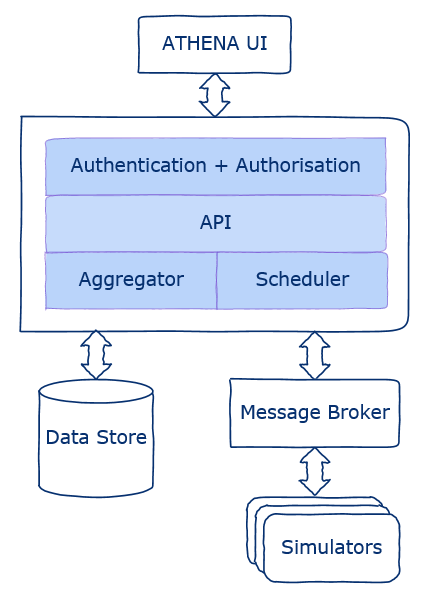
\includegraphics[width=0.4\textwidth]{Figures/ATHENA_conceptual_architecture}
\decoRule
\caption[ATHENA Conceptual Architecture]{Conceptual view of the multi-tier component architecture of the ATHENA system}
\label{fig:conceptArch}
\end{figure}

A user interface (UI), accessible via a web browser, provides access to the underlying modelling and simulation system. The user interface communicates with the backend system via REST\footnote{Representational State Transfer} API\footnote{Application Programming Interface} calls. These backend API calls are intercepted by an authentication and authorization layer, which perform user access control (ACL\footnote{Access Control List}) checks before despatching to various API endpoints. The backend system communicates with databases for the purpose of data persistence.

Apart from these traditional layers described above, the backend also communicates with a message broker for managing compute-intensive simulation tasks -- Bag-of-Tasks job execution using Enterprise Integration pattern --  Producer-Consumer Message-oriented architecture. These tasks are performed by a distributed set of workers, each hosting ATHENA's simulation engine.
\\
\\
%\subsection{Technology Stack}
\textbf{Technology Stack:} \quad Figure~\ref{fig:techStack} depicts ATHENA's technology stack. The backend service is a Spring framework-based modular application, written in Java. Primarily, the backend service provides logic related to the strategic aircrew training continuum, managing interfaces, business logic, data persistence, and distributed computation tasks. The data layer is composed of PostgreSQL RDBMS\footnote{Relational Database Management System}, which stores access control data, and document-oriented NoSQL MongoDB for storing all data related to the simulation model. Computation of simulations are performed by a network of lightweight workers, also written in Java, which communicate with the backend via JMS (Java Message Service). Apache ActiveMQ manages reliable delivery of messages containing simulation requests, results, and status updates. 

\begin{figure}
\centering
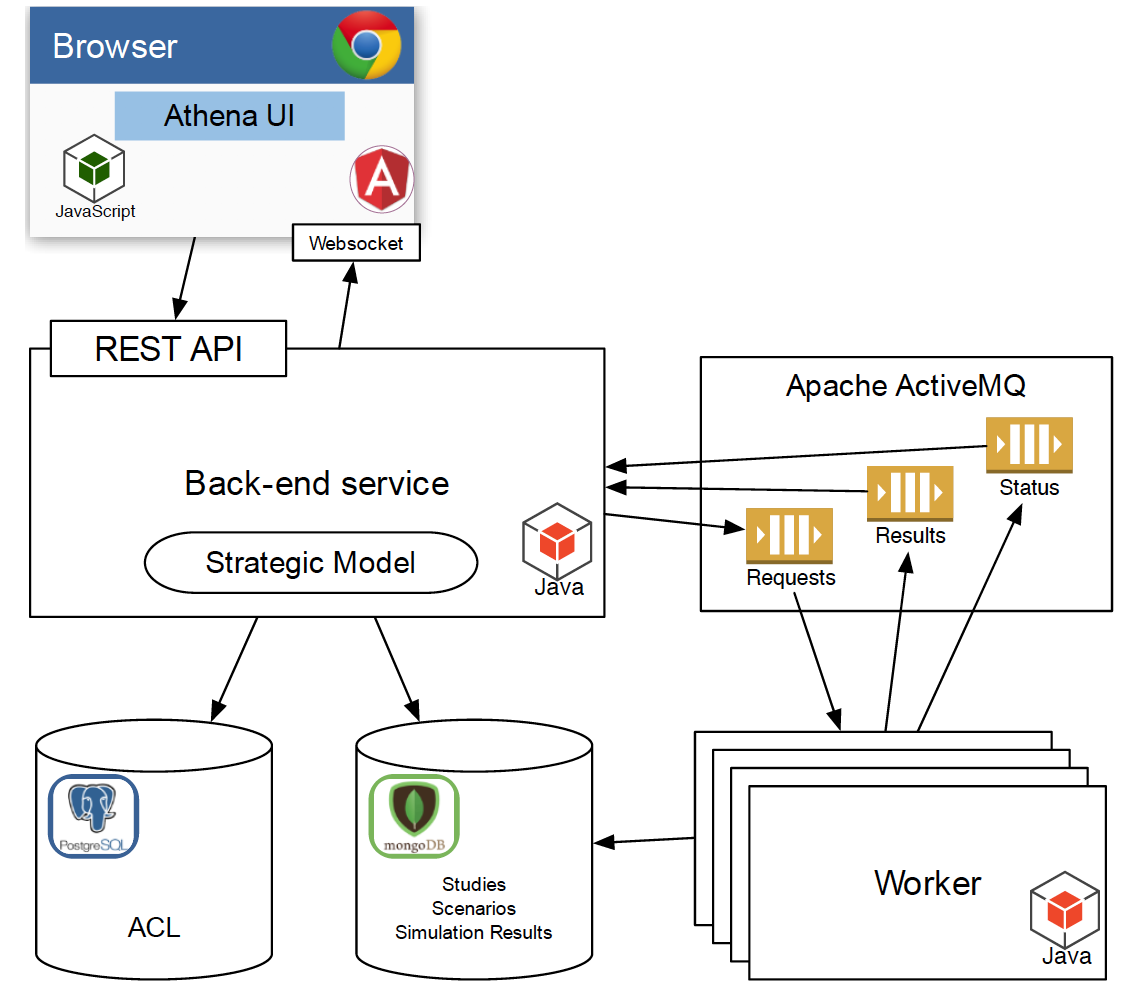
\includegraphics[width=0.5\textwidth]{Figures/ATHENA_tech_stack}
\decoRule
\caption[ATHENA Technology Stack]{ATHENA technology stack and their respective interactions}
\label{fig:techStack}
\end{figure}

The primary user interface is a AngularJS JavaScript Single-Page Application (SPA) loaded in an HTML5 compliant web browser. The UI communicates with the backend application server using both the HTTP REST API and WebSocket channels.

Figure~\ref{fig:scenarioScreen} shows a 10 year simulation result, the Scenario view which is the Sankey diagram\footnote{\url{https://en.wikipedia.org/wiki/Sankey_diagram}} (\textit{upper north}) -- visualisation of layered flow structure for the flow of the training continuum (\textit{left to right}). The Scenario Timeline (\textit{bottom south}) shows the statistical data of trainees or instructors over the whole simulation time span. The result also shows that the simulation have used \textbf{Monte Carlo} simulation and recruitment \textbf{optimisation algorithm} by labelling at the top left corner of the Sankey diagram.

\begin{figure}
\centering
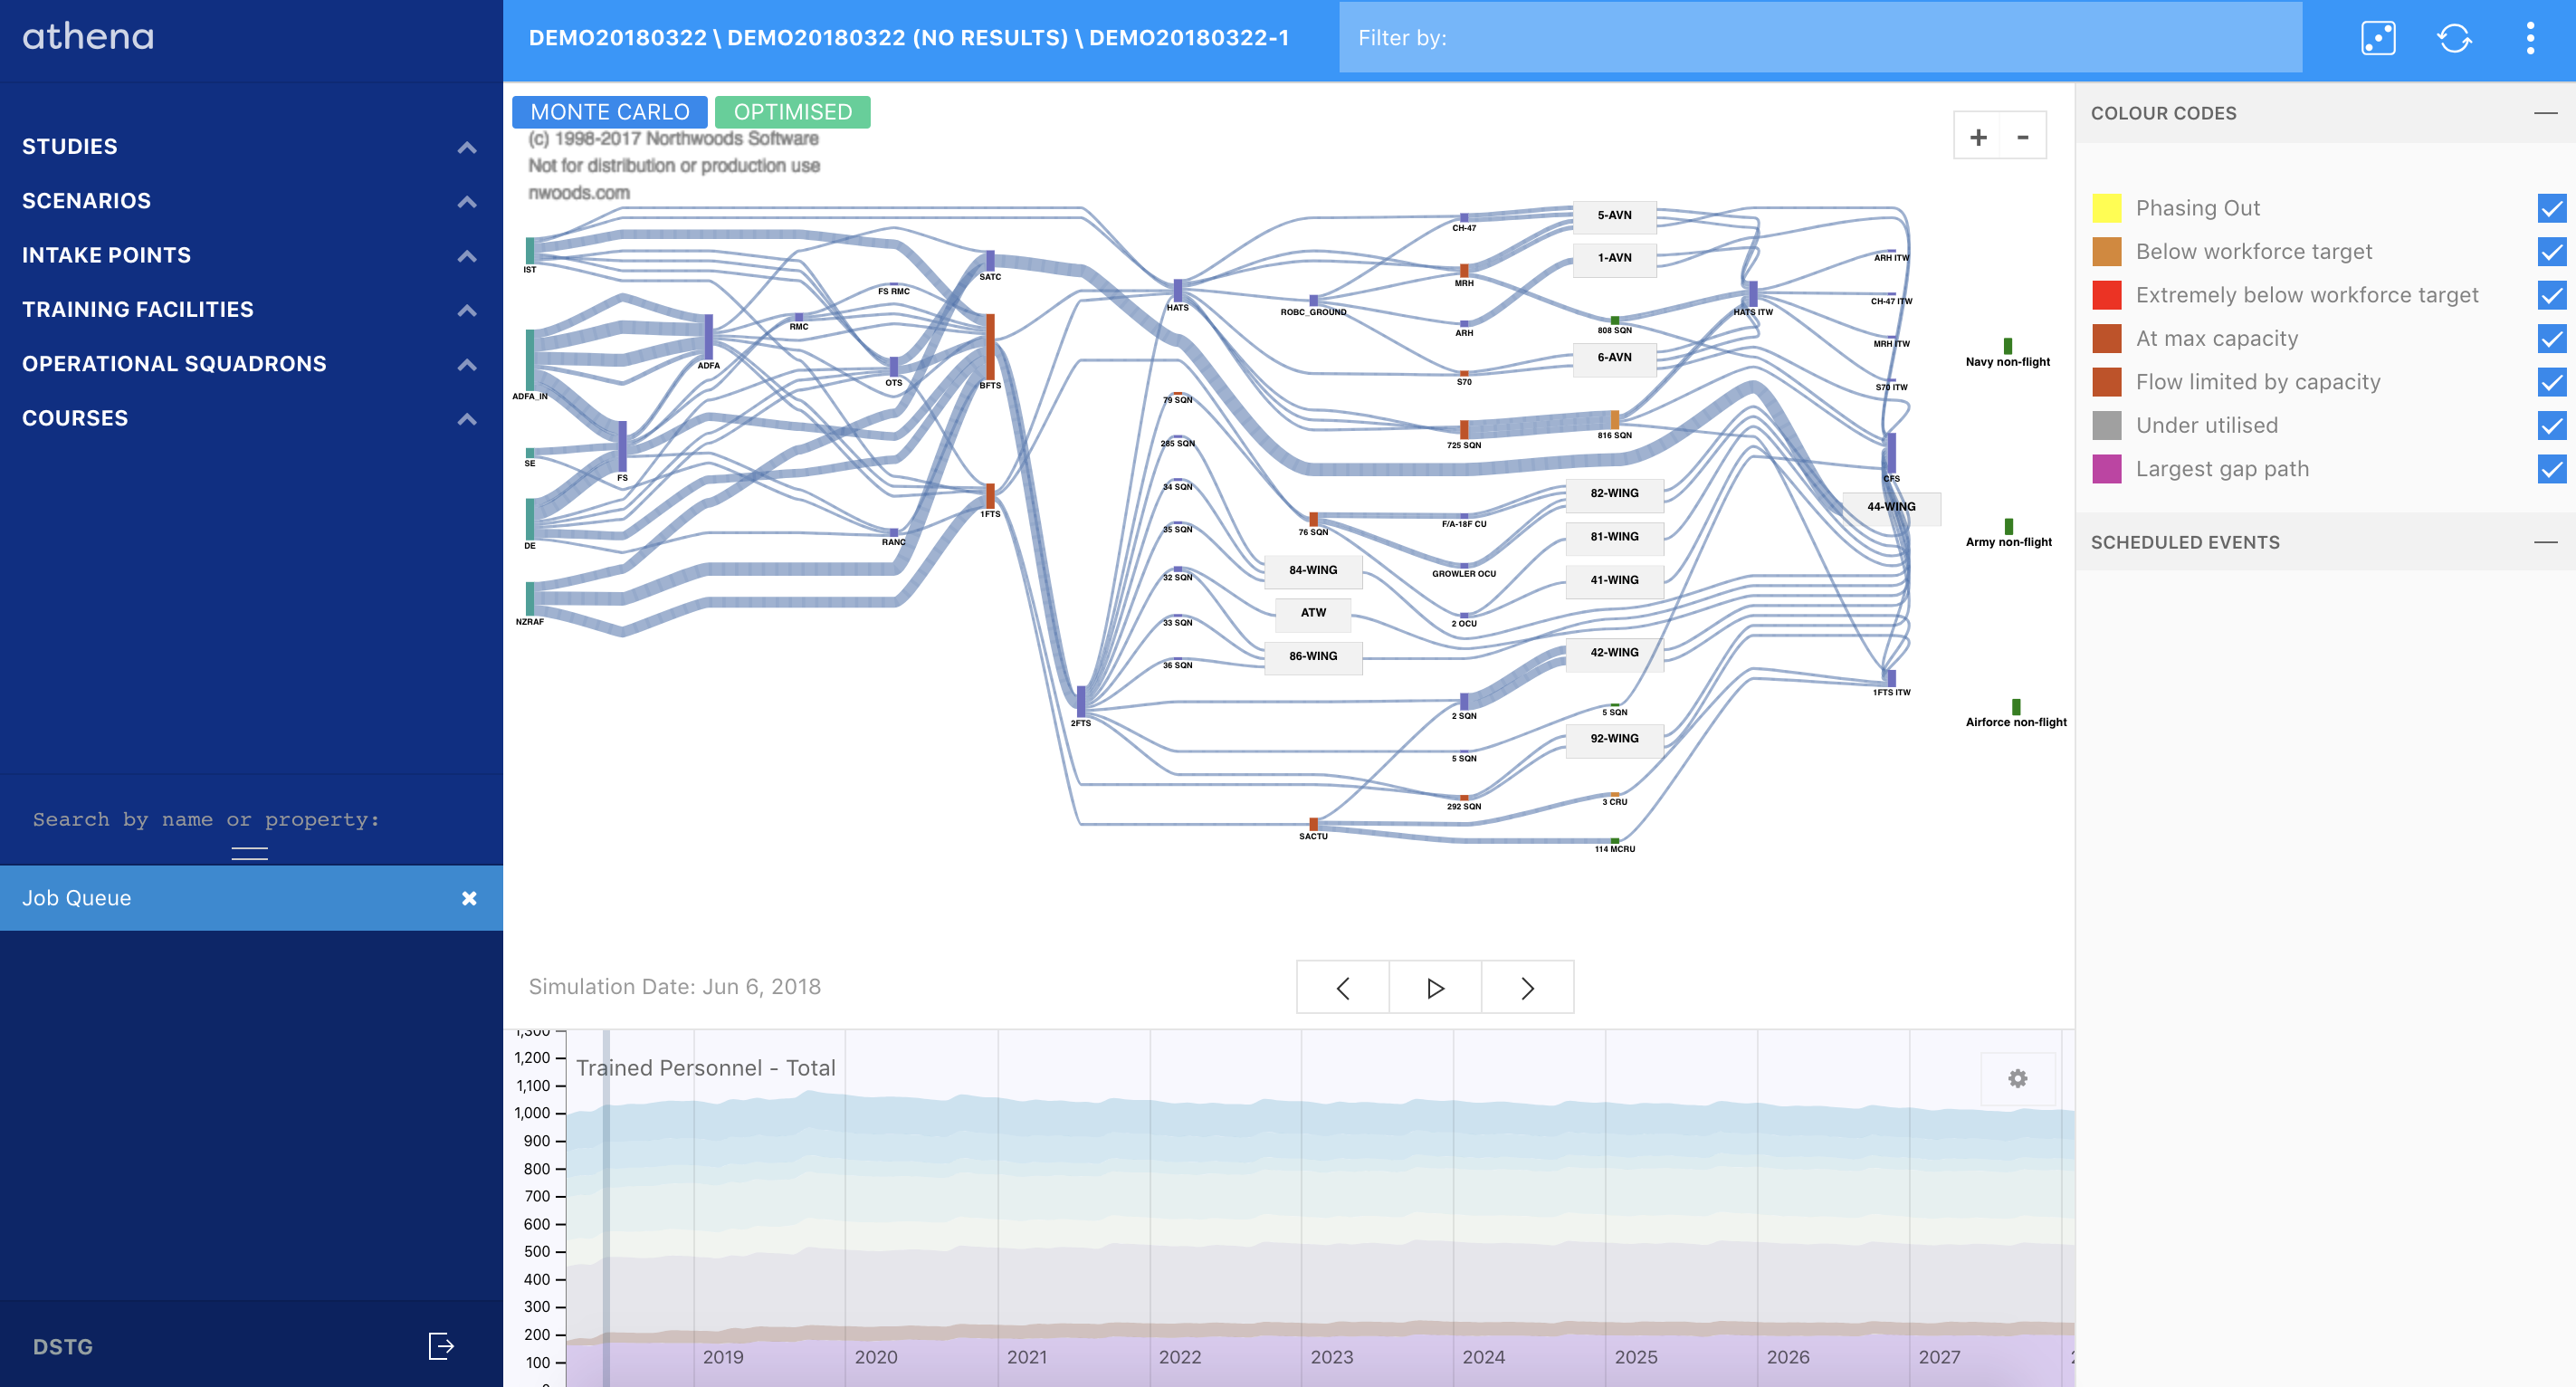
\includegraphics[width=0.8\textwidth]{Figures/ATHENA_scenario_screen}
\decoRule
\caption[ATHENA Scenario View]{ATHENA Scenario View}
\label{fig:scenarioScreen}
\end{figure}

\section{Remote Job Execution and Bag-of-Tasks Scaling Potential}

Simulation jobs can be computationally intensive, especially if one of the optimisation algorithms is activated. For this reason, a master-worker remote execution system has been designed aiming at offering high-performance and reliable simulations. Figure~\ref{fig:remoteJob} depicts this process.

\begin{figure}
\centering
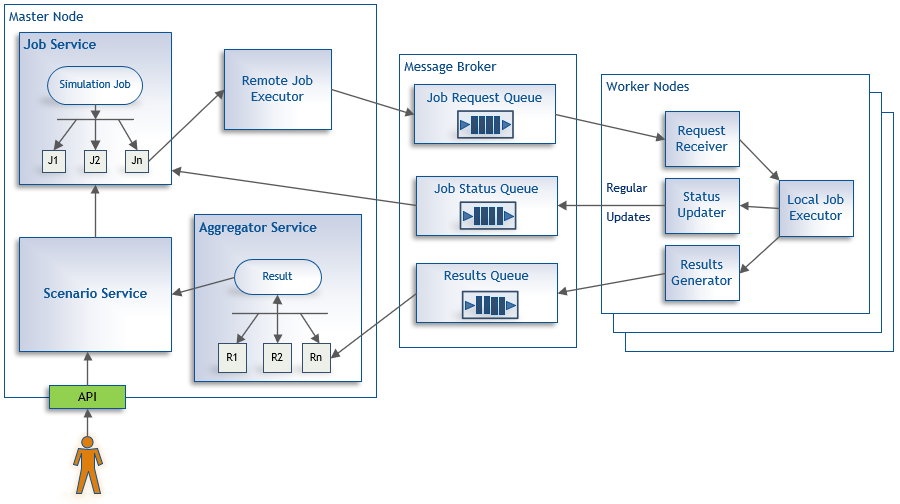
\includegraphics[width=0.8\textwidth]{Figures/ATHENA_remote_job_exec}
\decoRule
\caption[ATHENA Remote Job Execution]{ATHENA Process of remotely executing simulation jobs}
\label{fig:remoteJob}
\end{figure}

Monte-Carlo simulations, composed of many repetitions of the same process, are inherently a good fit for this system due to their embarrassingly parallel nature. 
In the master node, the job execution system is composed of a modular set of services. Once a scenario is submitted for simulation, the \textbf{Scenario Service} deals with assembling a simulation model with the correct inputs and creates one sub-scenarios for each Monte-Carlo repetition. Effectively, the simulation is parallelised into \textit{N} independent jobs, created by the \textbf{Job Service}, which is responsible for managing the job state, i.e. creating, updating and cancelling job executions. The \textbf{Remote Job Executor} interfaces with the \textbf{Message Broker} via the JMS protocol. At this point, the \textbf{Job Request Queue} will contain multiple job definitions, ready to be consumed by workers. 
There can be many worker nodes, which consume messages from the \textbf{Job Request Queue}, interpret the job definition, read job inputs, and perform local execution of the simulation model. As jobs are dequeued, start and finish execution, the worker sends status updates via the \textbf{Job Status Queue}, which are in turn consumed by the master in order to provided progress updates to the end-user. Each individual simulation repetition produces one result instance, or intermediate result. These are send via the \textbf{Results Queue} and consumed by an \textbf{Aggregator Service} that performs statistical aggregation, thus producing the mean and confidence intervals of all model statistics over all simulation runs. The execution is reliable in the sense that the failure of a worker does not cause the entire simulation to fail, as failed jobs are simply retried by another available worker. 
\\
\\
\\
For further details, readers are recommended to read the complete documentations of the ATHENA system in \parencite{athenaAllDoc}.
 
\chapter{Deployment: Containerisation and Scaling}

\label{Chapter3}

\section{Overview}
This chapter discuss as the evolution of ATHENA deployment approaches, address the scaling aspect and improvement done on each iteration. The fundamental understanding of Docker technologies\footnote{\url{https://docs.docker.com/engine/docker-overview/}} is assumed.

\noindent \textbf{Concept:} \quad The following diagram~\ref{fig:deployStack} depicts the one logical deployment of the ATHENA system with no specifics on how to layout this onto computing resources e.g. it could be on one machine or broken down into multiple machines.

\begin{figure}[H]
\centering
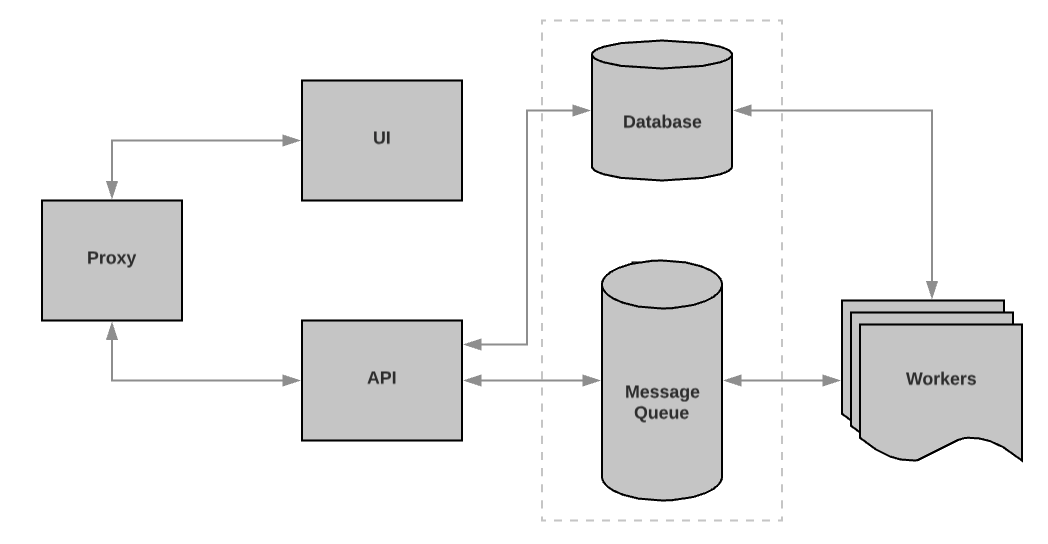
\includegraphics[width=0.5\paperwidth]{Figures/ATHENA_deploy_stack}
\decoRule
\caption[ATHENA Deployment Stack]{ATHENA Logical Deployment Stack}
\label{fig:deployStack}
\end{figure}

Contrary to typical lab or experimental setup that use for benchmarking or comparison purpose, the ATHENA deployment is, somewhat, in a real world setting and live deployments where users are actively using the system. The development and integral releases are pushing into the deployed sites regularly. Therefore, the deployment and operation consideration mainly favour stable steps and reliable approaches. Deployments are regularly snapshot and backed up. The server instance decommissioning are carefully planned and recycled when the machine vertical scaling is needed to replace the already provisioned environment. 

%\section{Infrastructure}
\noindent \textbf{Infrastructure:} \quad The Australian National eResearch Collaboration Tools and Resources (NeCTAR) is the federally funded research cloud platform where the underlying datacenters span across Australia capital cities. At present, it supports 6000+ virtual machines using around 30,000+\footnote{\url{https://status.rc.nectar.org.au/growth/infrastructure/}} vCPUs across Australia.

ATHENA uses NeCTAR as the main Infrastructure-as-a-Service (IaaS) Cloud provider. NeCTAR infrastructure is implemented and managed using the OpenStack cloud computing framework. The ATHENA deployment is leveraging across two tenancies with total number of 300 vCPU cores allocated for the project. The typical choice of instance size is between \textbf{m1} and \textbf{m2} flavours of \textbf{large}, \textbf{xlarge} \footnote{\url{https://support.ehelp.edu.au/support/solutions/articles/6000055380-resources-available-to-you}} ranging between 4 cores to 16 cores. The choice of base image is \textit{NeCTAR Ubuntu 16.04 LTS (Xenial) amd64}.

The ATHENA source code version control is hosted on Microsoft Visual Studio Team Services (VSTS)\footnote{\url{https://www.visualstudio.com/team-services}}. The deployment is mainly driven by Git Workflow\footnote{\url{https://git-scm.com/book/en/v2/Git-Branching-Branching-Workflows}}, VSTS's build and release pipelines. The VSTS's \textbf{Continuous Integration} (CI) and \textbf{Continuous Delivery} (CD) \parencite{httermann2012devops} are setup to push to the target deployment environments. The terms \textbf{DEV}, \textbf{STAGING} and \textbf{PROD} in Figure~\ref{fig:deployVSTS} represent the development, staging and production deployment environments of the ATHENA software stack. Build-agents are the VSTS build slaves for compiling and building the ATHENA artifacts.

\begin{figure}[H]
\centering
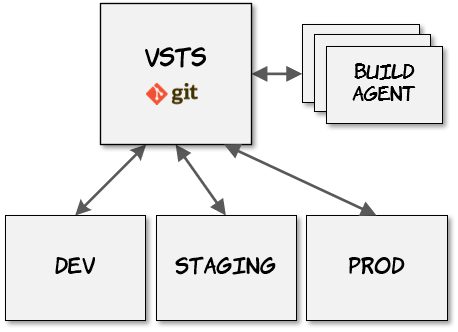
\includegraphics[width=0.3\paperwidth]{Figures/ATHENA_deploy_vsts}
\decoRule
\caption[ATHENA VSTS and Git]{ATHENA VSTS and Git Driven Deployment}
\label{fig:deployVSTS}
\end{figure}

\section{Containerised Deployment and Scaling}

Initially, the ATHENA stack was deployed in a good old-way of using distro packaging tool \verb|apt-get| and running using \verb|systemd/init.d| daemon services. This has performed through SSH terminal session on the node, e.g:

\begin{small}
\begin{lcverbatim}
apt install mongo
systemctl start mongod
\end{lcverbatim}
\end{small}

\noindent \textbf{IaC Automation Tool:} \quad Nonetheless, this were later change to use Ansible\footnote{\url{https://www.ansible.com}} as IaC automation tool. This improve the scripted knowledge of what has made changes to the server over the system deployment life cycle. The Ansible Playbook scripts were written according to server role such as \verb|db-server.yaml|, \verb|api-server.yaml|, so on. The pros of Ansible are agentless and, its only dependency is SSH which comes in default with most Linux distribution. The cons side of Ansible is that it requires a bit more care to script it in idempotent way. Otherwise the side-effect is detrimental e.g the use of the following task would wipe \verb|vdd| block device each time Ansible script run.

\begin{small}
\begin{lcverbatim}
shell (or command): mkfs.xfs -f /dev/vdd
\end{lcverbatim}
\end{small}
 
For a quick comparison, Chef\footnote{\url{https://www.chef.io}} and SaltStack\footnote{\url{https://saltstack.com}} tools were evaluated as Ansible alternative. The SaltStack can operate in both agent and non-agent mode -- whereas in agentless, it operates as light weight as Ansible. Chef requires an agent to be installed on all the nodes in the cluster fleet which is an overhead. On the other hand, Chef gives the most controlled environment such as retaining the guarantee system state. A more in-depth comparison is off interest for this paper, but the next contender would be SaltStack. The justification is solely based in favour of the KISS principle -- \textit{\textbf{K}eep \textbf{I}t \textbf{S}imple and \textbf{S}traightforward}.

\noindent \textbf{Vertical Scaling Issue:} \quad Furthermore, in the beginning, the whole ATHENA stack Figure~\ref{fig:deployStack} was deployed onto the single environment i.e. one VM instance. The pros with this approach is almost zero network latency among software components communication. But it needs a powerful machine. The highest flavour we can request on NeCTAR is \textit{m1.xxlarge: 16 cores, 64GB RAM}, although the real-world experience shows that this is somewhat difficult to get allocation from NeCTAR, which is understandable for a shared research facility. Most importantly, this approach has the potential vertical scaling limit as if requires more resources in one box.

\noindent \textbf{Stateful and Stateless:} \quad The first step of scale out approach is to identify the \textbf{State} nature of the software stack and split between stateful and stateless components. In addition, the components are built into the docker images (i.e. dockerised) and run as containers. Figure~\ref{fig:deployDockerised} depicts the arrangement of this approach -- stateful database containers on \verb|db-server| node and, pseudo-stateless API, stateless UI and Worker containers on another node. The scaling is a bit easier now. However, this is still a single node container scaling for the worker's Bag-of-Tasks remote job execution discussed in Chapter \ref{Chapter2}.

\begin{small}
\begin{lcverbatim}
docker-compose -f docker-compose.yaml -f staging.yaml  --project-name=stg \
   --scale worker=2
\end{lcverbatim}
\end{small}

\begin{figure}[H]
\centering
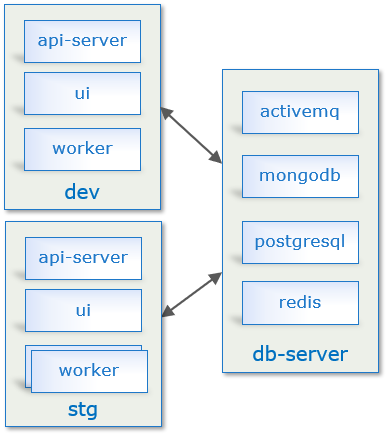
\includegraphics[width=0.4\textwidth]{Figures/ATHENA_dockerize}
\decoRule
\caption[ATHENA Dockerised]{ATHENA containerised and split by stateful and stateless components on different nodes}
\label{fig:deployDockerised}
\end{figure}

\noindent \textbf{Dedicated Workers:} \quad As discussed in Chapter \ref{Chapter2}, the ATHENA Worker's remote job execution and computation can become very CPU intensive when one of optimisation algorithms is activated in the simulated scenario. Further attempt to improve Worker's computation throughput, we can split the worker containers into a pool of worker nodes as shown in Figure~\ref{fig:dedicatedWorkers}. This solution is expensive but a good compromise if dedicated worker service is needed for QoS purpose.

\begin{figure}[H]
\centering
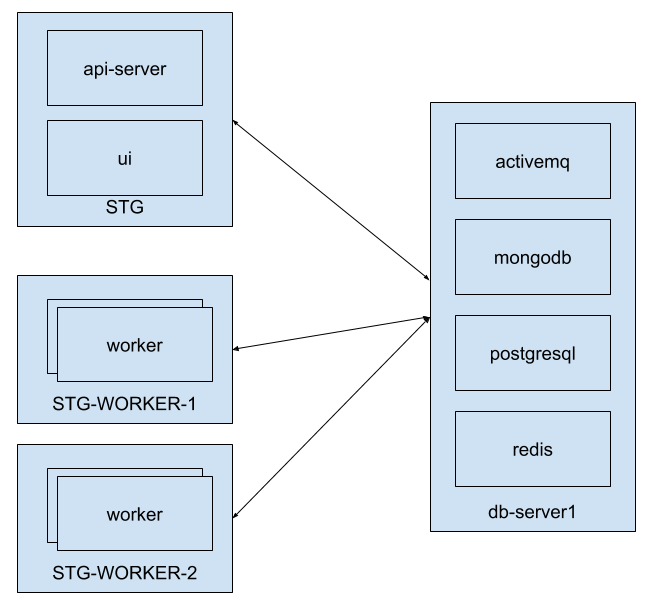
\includegraphics[width=0.4\textwidth]{Figures/ATHENA_dedicated_workers}
\decoRule
\caption[ATHENA Dedicated Workers]{ATHENA dedicated workers on different nodes to form pool of workers}
\label{fig:dedicatedWorkers}
\end{figure}

In fact, this dedicated workers approach is the recommended deployment for Production environment in the ATHENA Deployment Guide v1.0 \parencite{athenaAllDoc}. It requires network and resource provision as shown in Figure~\ref{fig:deployNetwork}. 

Note that, only ports 80 and 443 are exposed through the proxy-server to the external (public) network. The rest of the system resources form a trusted private network (subnet) among themselves and, is protected behind the firewall for all the ingress network traffic. The private network \verb|10.1.0.0/16| has setup and, a fixed static IP addressing is configured on each of the host systems. The host systems may have 2 NICs (network interface cards) typically eth0, eth1 and, have chosen 1 NIC for connecting this private internal network. The recommended network is Gigabit Ethernet (1GbE) or higher speed inter-network connection is assumed.

\begin{figure}[H]
\centering
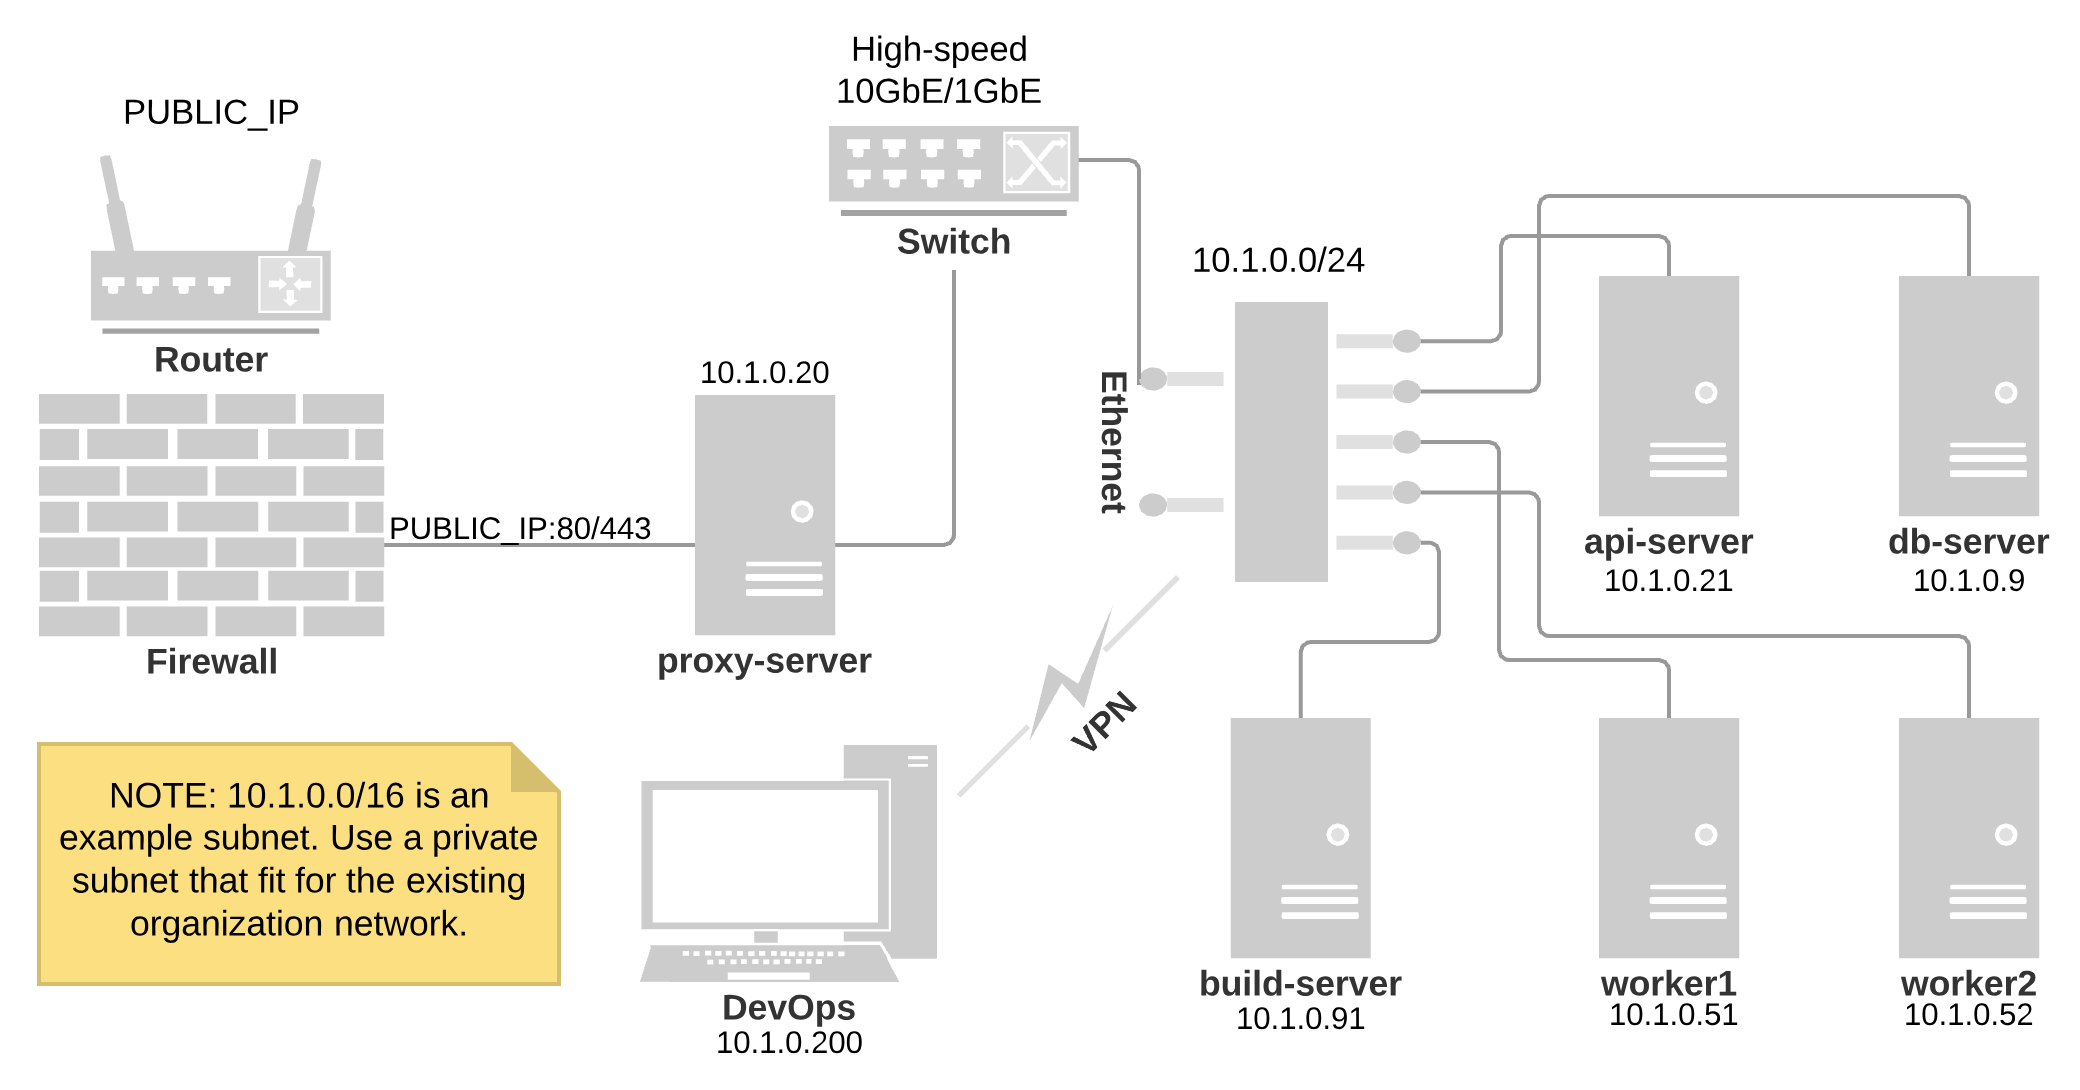
\includegraphics[width=0.7\paperwidth]{Figures/ATHENA_deploy_network_diagram}
\decoRule
\caption[ATHENA Network Diagram]{ATHENA Network Diagram}
\label{fig:deployNetwork}
\end{figure}

In this arrangement, we can horizontally scale out the system well. We can add more database nodes for MongoDB Sharding and Replication\footnote{\url{https://docs.mongodb.com/manual/}} to handle the terabytes (TB) of simulation data and, to retain these simulation data in the system for operational need. We can add more worker nodes into the dedicated worker pool for higher throughput. In ATHENA version 1.0, the api-server is still pseudo-stateless, in such that the Aggregator component as shown in Figure~\ref{fig:conceptArch} is required to aggregate all the results from the simulators computation. This has a potential bottleneck on the api-server. There is a plan to decompose the Aggregator component in a future ATHENA releases.

\section{Docker Swarm Mode}

To this point, we have identified how we can scale the ATHENA system at different layers. However, the system operator still requires to configure and manage these computing resources manually. A good estimated time to add a new worker with the prepared IaC automation scripts; plus NeCTAR VM instance spin up time takes around 20 to 30 minutes. And the operator will have to spin down the instances where there no need of computation demands and keep the system in minimal operational state. This entails the need for self-managed Autonomic Computing \parencite{1160055} and, the notion of autonomous cluster management and job execution platform from a pool of computing resources -- also refer as \textbf{Orchestrations} in a more recent deployment literature.

Since we have containerised the entire ATHENA software components, the next best thing is to switch into docker swarm mode. Turning into the docker swarm mode is relatively straight forward. On the chosen node, initialize the manager (master) and add (swarm) worker nodes to form docker swarm cluster. Service scaling is easy, however, the scaling instruction need to manually set it on the swarm manager node through CLI or docker-compose stack deployment \verb|service.[srv_name].deploy.replicas:5| nomenclature.
\begin{small}
\begin{lcverbatim}
docker swarm init --advertise-addr 192.168.99.100
docker swarm join --token SWMTKN-1-[tonken-scrap] 192.168.99.201:2377
docker swarm join --token SWMTKN-1-[tonken-scrap] 192.168.99.202:2377
docker node ls
ID                            HOSTNAME         STATUS          AVAILABILITY
[nxor..] *   swarm-master        Ready          Active          Leader
[ke35...]    swarm-worker1       Ready          Active
[u2wx...]    swarm-worker2       Ready          Active
docker service scale athena_worker=5
athena_worker scaled to 5
\end{lcverbatim}
\end{small}

For the intreset of the thesis length, the details review of how Docker Swarm works\footnote{\url{https://docs.docker.com/engine/swarm/how-swarm-mode-works/nodes/}} is left to its documentation. This thesis takes advantage of the related studies made within the \textit{\groupname}, of which studies \parencite{swarmKubeBench2} benchmarks on the performance and qualitative comparison of Docker Swarm and Kubernetes. There are also internet articles available on qualitative comparison of these two technologies e.g. Platform9\footnote{\url{https://platform9.com/blog/kubernetes-docker-swarm-compared/}}. 

Base on these literatures, we can conclude that the technical merit of both technologies is closely matched, however, in the context of the research presenting in this paper, the \emph{built-in Auto-scaling feature} in Kubernetes has ruled out for a probable auto-scaling solution for the ATHENA system. The justification to \emph{why Kubernetes} decision is somewhat empirical choice based on maturity of the software. It is also a pragmatic observation over adoption of Kubernetes trend by many Cloud providers and key players, e.g. Google, IBM, Azure, AWS, RedHat, and to name few. The technical insight in Chapter \ref{Chapter4} reinforces this hypothesis.

% \parencite{swarmKubeBench}
\chapter{Kubernetes: Insight and Auto-scaling}

\label{Chapter4} 

\section{Overview}

This chapter focus on the critical review and details setup of Kubernetes (k8s or Kube) cluster for deploying the auto-scalable ATHENA system. The Kubernetes key components are introduced, however, a more details and complete reference left it to the k8s official documentation\parencite{kubeDoc}.

With reference to the official website\footnote{\url{https://kubernetes.io}}, Kubernetes is the \emph{production grade container orchestration system that design for the deployment, scaling, management, and composition of application containers across clusters of hosts}. It is a robust container-management system that create a virtual abstraction layer on top of Cloud platform for deploying and maintaining scalable distributed systems. This abstraction enable users to deploy their applications consistently between different Cloud providers.

%Burns:2016:BOK:2898442.2898444

Kubernetes is the third incarnation of Google own container-management systems -- whereas the k8s is built upon its predecessors Borg and Omega \parencite{44843} systems over a decade experience of production run at scale. At Google with Borg system, \parencite{43438} reported that it \emph{runs hundreds of thousands of jobs, from many thousands of different applications, across a number of clusters each with up to tens of thousands of machines}. 

%In \parencite{Hightower:2017:KUR:3175917}, it claims that Google deploys over two billion application containers a week with Borg system. These figures are impressive but it comes in price. 

\section{Looking at Kube Design}
\label{kubeDesign}
From Borg-Omega to Kube, the Google software engineers learned lessons\parencite{44843} on how best to tackle with the container-management at design\footnote{\url{https://kubernetes.io/blog/2015/06/the-distributed-system-toolkit-patterns/}} and bring the architecture to next level\footnote{\url{https://kubernetes.io/blog/2016/06/container-design-patterns/}} to make it easy for developers to write the distributed applications and services that run in cloud and datacenter environments. Looking at Kubernetes, we can observe that the design of the system become more generic and abstraction compare to its predecessors. It goes beyond more than container-management. Since the process of containerisation encapsulates the application, Kubernetes introduces \textit{Application-Oriented Infrastructure} (AOI) with two motivations:
\begin{itemize}
\item abstracting away details of machine and operating system from application developer and deployment
\item \emph{single application process per container} Design Pattern entails that managing containers mean managing applications, therefore, it shifts the Kube API from machine-oriented to application-oriented and, improves application deployment and introspection 
\end{itemize}

\noindent\textbf{Objects Management:} \quad To model a generalised system is a challenging goal for every distributed system designer. To realise this generalisation, at very abstract, Kubernetes is just a \textbf{Objects Management} API service. The Kubernetes API does not perform the functional aspect of the system, but the objects its managed deliver these functionality. In Kubernetes, we can define the type of what kind, which does something. The shape of the Kubernetes Object can be expressed in YAML format. The mandatory fields for a Kubernetes Object are summarised in Table~\ref{kubeObjectTable}.

\begin{table}[H]
\centering
    \begin{tabular}{ | l | p{11cm} |}
    \hline
    Field & Description \\ \hline
    apiVersion & Which version of the Kubernetes API using to create this object. \\ \hline
    kind & What kind of object you want to create. \\ \hline
    metadata & Data that helps uniquely identify the object, including a name string, UID, and optional namespace. \\ \hline
    spec & To Describe the desired state of the object. Precise format of the object spec is different for every Kubernetes object, and contains nested fields specific to that object. \\ \hline
    status & Provides read-only information about the current state of the object, is supplied and updated by the Kubernetes system. Like spec, format is vary by object type. \\
    \hline
    \end{tabular}
\caption{Kubernetes Object Mandatory Fields}
\label{kubeObjectTable}
\end{table}

\noindent\textbf{Work Out:} \quad To understand how Objects Management work in Kubernetes API, we will go through a quick exercise. Consider we have Kubernetes and its API service up and running. Consider we like to create an object of type, say, \ctexttt{FireBall}. Create a YAML as follows.

\begin{lcverbatim}
apiVersion: apiextensions.k8s.io/v1beta1
kind: CustomResourceDefinition
metadata:
  name: fireball.sankholin.com
spec:
  group: fireball.sankholin.com
  version: v1
  scope: Namespaced
  names:
    plural: fireballs
    singular: fireball
    kind: FireBall
    shortNames: 
    - fb
    - FB
\end{lcverbatim}

\noindent And create this \ctexttt{FireBall} type in Kube API:
\begin{lcverbatim}
kubectl create -f  CRD_Fireball.yaml
\end{lcverbatim}

\noindent And now we can prescribe our \ctexttt{FireBall} type in YAML as follows. Notice of \emph{kind} field.

\begin{lcverbatim}
apiVersion: "fireball.sankholin.com/v1"
kind: FireBall
metadata:
  name: my-fireball-object
spec:
  image: sankholin.com/fireball-container-image:latest
\end{lcverbatim}

\noindent Finally, create an instance of \ctexttt{FireBall} object.
\begin{lcverbatim}
kubectl create -f my-fireball.yaml
\end{lcverbatim}

\noindent This will pull and deploy the containerised \emph{FireBall} application image from \emph{Container Image Registry}. The use of \textit{FireBall} nomenclature is intentional and the exact behaviour of what \emph{FireBall} type might do is left it for reader interpretation -- e.g. a cluster of Game engine API. This is to show that how Kube API handle custom resources in a generic way through \ctexttt{CustomResourceDefinitions}. Kube Objects are persistent entities (i.e. CRUD\footnote{Create, Read, Update, Delete}) which represent the state of the cluster. In this exercise, we are using \ctexttt{CustomResourceDefinition} which is one of the built-in resource type of Kube API which purpose is to be able to create a \textit{Custom Resources} inside Kube system. Table~\ref{kubeBuiltinResources} summarise the commonly use Kubernetes built-in Resources\footnote{Resource as in REST API} (or \emph{kind}).

\begin{table}[H]
\centering
    \begin{tabular}{ | l | p{12cm} |}
    \hline
    Kind & Description \\ \hline
    \href{https://kubernetes.io/docs/concepts/workloads/pods/pod-overview/}{Pod} & The basic building block of Kubernetes -- the smallest and simplest unit in the Kubernetes object model. \\ \hline
    \href{https://kubernetes.io/docs/concepts/services-networking/service/}{Service} & Service is an abstraction which defines a logical set of Pods and a policy by which to access them - sometimes called a micro-service. \\ \hline
    \href{https://kubernetes.io/docs/concepts/workloads/controllers/replicaset/}{ReplicaSet} & Next-generation Replication Controller. A ReplicaSet ensures that a specified number of pod replicas are running at any given time. \\ \hline
    \href{https://kubernetes.io/docs/concepts/workloads/controllers/deployment/}{Deployment} & Deployment controller provides declarative updates for Pods and ReplicaSets. You describe a desired state in a Deployment object, and the Deployment controller changes the actual state to the desired state at a controlled rate. \\ \hline
    \href{https://kubernetes.io/docs/concepts/workloads/controllers/statefulset/}{StatefulSets} & StatefulSet is the workload API object used to manage stateful applications. \\ \hline
    \href{https://kubernetes.io/docs/concepts/workloads/controllers/daemonset/}{DaemonSet} & A DaemonSet ensures that all (or some) Nodes run a copy of a Pod. As nodes are added to the cluster, Pods are added to them. As nodes are removed from the cluster, those Pods are garbage collected. \\ \hline
    \href{https://kubernetes.io/docs/concepts/workloads/controllers/jobs-run-to-completion/}{Job} & A job creates one or more pods and ensures that a specified number of them successfully terminate. \\ \hline
    \href{https://kubernetes.io/docs/concepts/workloads/controllers/cron-jobs/}{CronJob} & A Cron Job manages time based Jobs, run: Once or Repeatedly at a specified point in time. \\
    \hline
    \end{tabular}
\caption{Kubernetes Built-in Resources}
\label{kubeBuiltinResources}
\end{table}

Note that Table~\ref{kubeBuiltinResources} is just introductory Kubernetes resources that need to get started work on with the Kubernetes in most use cases. For the interest of thesis length, it is recommended to read Kubernetes documentation \parencite{kubeDoc} for how these built-in Kubernetes resources work in specific to their functionality.

\section{Tackling at Production Ready Setup}

Kubernetes is a much more complex system to up and run with -- it is quite a daunting task for setting up \emph{Production Ready} Kubernetes deployment for user's own on-premise, bare-metal or Private Cloud infrastructure. It has steep learning curve. Its breadth of functionality grows daily, documentation is outdated quickly and is enough to overwhelm even the most advanced users. Every layer of Kubernetes have a couple of different ways to setup and options to pick. Nevertheless, Kubernetes composes of components for \textbf{Master} role and components for the \textbf{Node} role. Table~\ref{kubeMasterComp} and Table~\ref{kubeNodeComp} summarise this. These components are fundamental executables for up and running the Kubernetes cluster. 

\begin{table}[H]
\centering
    \begin{tabular}{ | l | p{10cm} |}
    \hline
    Component & Description \\ \hline
    \href{https://kubernetes.io/docs/reference/command-line-tools-reference/kube-apiserver/}{kube-apiserver} & exposes the API and the front-end for the Kubernetes control plane \\ \hline
    \href{https://kubernetes.io/docs/reference/command-line-tools-reference/kube-scheduler/}{kube-scheduler} & monitor newly created pods and selects a node for them to run on \\ \hline
    \href{https://kubernetes.io/docs/reference/command-line-tools-reference/kube-controller-manager/}{kube-controller-manager} & control loop that watches the shared state of the cluster through the apiserver and makes changes attempting to move the current state towards the desired state \\ \hline
    \href{https://kubernetes.io/docs/tasks/administer-cluster/configure-upgrade-etcd/}{etcd} & consistent and highly-available key value store backing for all cluster data \\
    \hline
    \end{tabular}
\caption{Components for Kubernetes Master Role}
\label{kubeMasterComp}
\end{table}

\noindent \textbf{Hard Way:} \quad For straight forward approach, we could spin up one node and install all the components mention in Table~\ref{kubeMasterComp} to run as Kube Master role. And spin up one or more nodes to install all the components mention in Table~\ref{kubeNodeComp} to run as Kube Node role. Since Kubernetes is written in GoLang\footnote{\url{https://golang.org}}, we could download the source -- compile, build -- or download pre-compiled binary and run executables in foreground or wrap into \verb|systemd| daemon services. This would work in principle, at least. However so, this has to deal with more low level handling and, generally \emph{"goto"} setup for a Kube developer.

\begin{table}[H]
\centering
    \begin{tabular}{ | l | p{11cm} |}
    \hline
    Component & Description \\ \hline
    \href{https://kubernetes.io/docs/reference/command-line-tools-reference/kubelet/}{kubelet} & An agent that runs on each node in the cluster. It makes sure that containers are running in a pod. \\ \hline
    \href{https://kubernetes.io/docs/reference/command-line-tools-reference/kube-proxy/}{kube-proxy} & enables the Kubernetes service abstraction by maintaining network rules on the host and performing connection forwarding \\  \hline
    container-runtime & the software that is responsible for running containers -- supports several runtimes: \textbf{Docker}, \textbf{rkt}, \textbf{runc} and any Open Container Initiative (OCI) runtime specification implementation \\
    \hline
    \end{tabular}
\caption{Components for Kubernetes Node Role}
\label{kubeNodeComp}  
\end{table}

\noindent \textbf{Streamline Toolkit:} \quad Up and running in \emph{Hard Way} is not an ideal for \emph{Production Ready} setup. For this purpose, Kube community has diverse range of streamline solution for many different setup that are specifics to Public Cloud Provider, Linux distro, and so on. Table~\ref{kubeToolkits} summarise the recommended toolkit selection for setting up Kube cluster. 

\begin{table}[H]
\centering
    \begin{tabular}{ | l | p{12cm} |}
    \hline
    Toolkit & Description \\ \hline
    \href{https://kubernetes.io/docs/setup/independent/create-cluster-kubeadm/}{kubeadm} & bootstrap a best-practice Kubernetes cluster in an easy, reasonably secure and extensible way. \textbf{Kubernetes Certified}. \\ \hline
    \href{https://github.com/kubernetes-incubator/kubespray}{Kubespray} & install a Kubernetes cluster hosted on GCE, Azure, OpenStack, AWS, or Baremetal. Ansible. \\  \hline
    \href{https://github.com/kubernetes/kops}{kops} & helps you create, destroy, upgrade and maintain production-grade, highly available, Kubernetes clusters from the command line for AWS \\
    \hline
    \end{tabular}
\caption{Toolkits for Streamline Kubernetes Cluster Setup as of v1.10}
\label{kubeToolkits}
\end{table}

The kubeadm is chosen to bootstrap the Kube cluster for the purpose of ATHENA deployment. However, also note that, Kubernetes documentation offer dozens of different way\footnote{\url{https://kubernetes.io/docs/setup/pick-right-solution/}} to setup Kube cluster. This research finds that kubeadm is the most appropriate toolkit for setting up \emph{Production Ready} Kubernetes cluster. The justification for \emph{why kubeadm} is because it is the Kubernetes Certified Solution as of v1.10, its abstraction to IaC automation tool and it can streamline the upgrade of the Kube cluster reliably.

\begin{small}
\begin{lcverbatim}
root@athena-kube-master1:~# kubeadm upgrade plan
[preflight] Running pre-flight checks.
[upgrade] Making sure the cluster is healthy:
(scrap)
Components that must be upgraded manually after you have upgraded the \
   control plane with 'kubeadm upgrade apply':
COMPONENT   CURRENT      AVAILABLE
Kubelet     4 x v1.9.4   v1.10.2

Upgrade to the latest stable version:
COMPONENT            CURRENT   AVAILABLE
API Server           v1.9.4    v1.10.2
Controller Manager   v1.9.4    v1.10.2
Scheduler            v1.9.4    v1.10.2
Kube Proxy           v1.9.4    v1.10.2
Kube DNS             1.14.7    1.14.7
Etcd                 3.1.11    3.1.11

You can now apply the upgrade by executing the following command:
	kubeadm upgrade apply v1.10.2
Note: Before you can perform this upgrade, you have to update kubeadm to v1.10.2.

_____________________________________________________________________

root@athena-kube-master1:~# apt-get install --only-upgrade kubeadm
(scrap)
root@athena-kube-master1:~# kubeadm upgrade apply v1.10.2
(scrap)
\end{lcverbatim}
\end{small}

\noindent Figure~\ref{fig:kubeadm} shows the result of Kubernetes components installed into Master and Node role respectively using kubeadm. 

\begin{figure}[H]
\centering
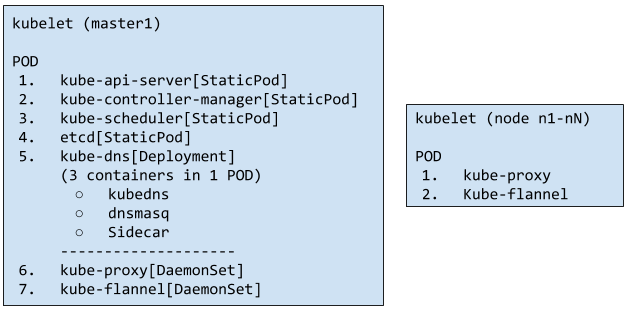
\includegraphics[width=0.55\paperwidth]{Figures/KUBE_kubeadm}
\decoRule
\caption[Kubebernetes Components on Master and Node]{Kubebernetes Components on Master and Node using kubeadm}
\label{fig:kubeadm}
\end{figure}

\noindent It is interesting to observe that at the basic bootstrapping for \textbf{a Kube Node} means a machine installed with \textbf{just kubelet component and container runtime engine}. After kubelet and Docker container runtime engine installed, up and and running as a \verb|systemd| daemon service, a Pod can be deployed. Therefore, Figure~\ref{fig:kubeadm} shows that api-server, controller-manager, scheduler, etcd components are running as Pods on a node with Master role; and similarly kube-proxy is running as Pod on both Master and Node roles.

Recall Table~\ref{kubeBuiltinResources} that a Pod is the built-in resource type (a \emph{kind}) and the basic unit of Kubernetes Object model. In this case, the kube-api-server, a GoLang application is containerised and deployed as a Pod. The \verb|kube-apiserver.yaml| manifests as follows.

\begin{lcverbatim}
apiVersion: v1
kind: Pod
metadata:
  labels:
    component: kube-apiserver
    tier: control-plane
  name: kube-apiserver
  namespace: kube-system
spec:
  containers:
  - command:
    - kube-apiserver
    image: gcr.io/google_containers/kube-apiserver-amd64:v1.10.2
    (scrap)
\end{lcverbatim}

However, note that, kubeadm created the kube-apiserver component as a special Pod type called Static Pod. From k8s documentation\footnote{\url{https://kubernetes.io/docs/tasks/administer-cluster/static-pod/}}, \parencite{kubeDoc} states that \emph{Static Pods are managed directly by kubelet daemon on a specific node, without the API server observing it. Kubelet automatically creates so-called mirror pod on the Kubernetes API server for each static pod, so the pods are visible there, but they cannot be controlled from the API server}. From this, we can also observe that kubelet can directly bootstrap a Pod, and it shares the Kubernetes Objects Management with the kube-apiserver to sudden extent.

\subsection{Add-ons}

In addition to the Kubernetes Master and Node components (Tables~\ref{kubeMasterComp}, \ref{kubeNodeComp}), we can also observe that there are kube-dns on Master role and, kube-flannel running on both Master and Node role. These components are called \textbf{Add-ons}\footnote{\url{https://kubernetes.io/docs/concepts/cluster-administration/addons/}} which extend the functionality of Kubernetes. Table~\ref{kubeadmAddons} summarise components that are deployed as part of the bootstrapping Kubernetes cluster by \verb|kubeadm init|\footnote{\url{https://kubernetes.io/docs/reference/setup-tools/kubeadm/kubeadm-init/}}.

\begin{table}[H]
\centering
    \begin{tabular}{ | l | p{11cm} |}
    \hline
    Add-ons & Description \\ \hline
    kube-dns & The internal implementation for Kubernetes DNS service. \\ \hline
    kube-flannel & Flannel\footnote{\url{https://github.com/coreos/flannel}} is an overlay network provider that can be used with Kubernetes Pod network. \\ 
    \hline
    \end{tabular}
\caption{Additional components deployed by kubeadm init}
\label{kubeadmAddons}  
\end{table}

\noindent To bootstrap the full-fledge \emph{Production Ready} Kubernetes cluster, there are compulsory add-ons such as like these. Note though that, Kubernetes documentation \parencite{kubeDoc} offer a dozens of Add-ons\footnote{\url{https://kubernetes.io/docs/concepts/cluster-administration/addons/}}; some of which are competing technologies and alternatives for the particular functionality e.g. to use \textbf{Weave Net} instead of \textbf{Flannel} for Pod Networking.

\subsection{Pod Networking}

From Table~\ref{kubeadmAddons}, there is a notion of \emph{Overlay Network}. In Kubernetes, the concept of Pod is to encapsulates containers. A Kube Pod object holds one or more containers, and introduces IP-per-Pod for network model. It implies IP addresses at the Pod scope. Therefore, containers within a Pod share their network namespaces including their IP address. The Pod networking requirement\parencite{kubeDoc} states that nodes and containers can communicate with all other containers \textbf{without NAT} and, the IP that a container sees itself as is the same IP that others see it as. In a nutshell, Kubernetes network model imposes barring any NAT -- intentional network segmentation policies. Kubernetes documentation offers a dozen of different way\footnote{\url{https://kubernetes.io/docs/concepts/cluster-administration/networking/}} for implementing this networking requirement -- Overlay Network is one of them. The implementation usually offer as \emph{Add-ons}, however, it is a compulsory step. Medium articles by google-cloud\footnote{\url{https://medium.com/google-cloud/understanding-kubernetes-networking-pods-7117dd28727}}, ApsOps\footnote{\url{https://medium.com/@ApsOps/an-illustrated-guide-to-kubernetes-networking-part-2-13fdc6c4e24c}} illustrated details on how Overlay Network is used for Kubernetes Pod networking requirement.

For the context of \emph{compute auto-scaling research} presenting in this thesis, the further investigation on performance comparison of Pod Networking with competing technologies left out for future work.

\subsection{Service}
\label{kubeService}
\noindent \textbf{Service Proxies:} \quad In Kubernetes, Pods are ephemeral and mortal. This is due to the fact that the Kube cluster can replicate Pod, dynamically scale up or down, self-healing and self-managing. As the Pod get destroyed or recycled, the Pod IP address may change. This is not the desire effect for the application developer to keep track of these IP addresses. Service is an network abstraction layer to retain the consistent endpoint within the cluster. Service can be also seen as frontend service proxies for other Kubernetes objects such as Pod, Deployment, ReplicaSet, etc. For the implementation, kube-proxy is responsible for creating a form of Virtual IP in 3 different proxy modes -- userspace, iptables, IPVS --  for Services of type other than ExternalName. For publishing services, it offers 4 different types as summarise in Table~\ref{kubeServiceTypes}.

\begin{table}[H]
\centering
    \begin{tabular}{ | l | p{11cm} |}
    \hline
    Type & Description \\ \hline
    ClusterIP & Exposes the service on a cluster-internal IP. \textbf{Default type}. \\ \hline
    NodePort & Exposes the service on each Node’s IP at a static port. \\  \hline
    LoadBalancer & Exposes the service externally using a cloud provider’s load balancer. \\ \hline
    ExternalName & Maps the service to the contents of the externalName field (e.g. foo.bar.example.com), by returning a CNAME record with its value. \\
    \hline
    \end{tabular}
\caption{Kubernetes service types for publishing service endpoints}
\label{kubeServiceTypes}  
\end{table}

\noindent \textbf{Service Discovery:} \quad For Service Discovery purpose, Kubernetes runs internal DNS. This comes in as \textbf{Add-ons}, however, compulsory. Kubeadm deployed kube-dns\footnote{\url{https://kubernetes.io/docs/tasks/administer-cluster/dns-custom-nameservers/}} Pod for this purpose. For example, the following \verb|athena-ui.yaml| service manifest creates a service endpoint for the athena-ui.

\begin{small}
\begin{lcverbatim}
apiVersion: v1
kind: Service
metadata:
  labels:
    app: athena-ui
  name: athena-ui
spec:
  ports:
    - port: 80
  selector:
    app: athena-ui
\end{lcverbatim}
\end{small}

\noindent The following screenshot shows ATHENA's components and their service proxies setup. 

\begin{small}
\begin{lcverbatim}
root@athena-kube-master1:~# kubectl get svc
NAME                TYPE        CLUSTER-IP       EXTERNAL-IP   PORT(S)   AGE
athena-analytics    ClusterIP   10.103.197.212   <none>        80/TCP    61d
athena-api-server   ClusterIP   10.101.72.108    <none>        80/TCP    54d
athena-ui           ClusterIP   10.103.117.69    <none>        80/TCP    82d
\end{lcverbatim}
\end{small}

\noindent In this example, we can say that, the athena-ui.yaml service manifest created a DNS
\\
\verb|athena-ui.default.svc.cluster.local|
\\
that resolve to the Service Endpoint IP address \verb|10.103.117.69|.
\\
\\
\noindent \textbf{Exposing Service Endpoint:} \quad We can reach to the service's \textbf{ClusterIP}, from all nodes within cluster, e.g:

\begin{small}
\begin{lcverbatim}
root@athena-kube-master1:~# curl -s --user (scrap):(scrap) 10.101.72.108/api/version
{"version":"1.0.1-SNAPSHOT"}
root@athena-kube-n1:~# curl -s --user (scrap):(scrap) 10.101.72.108/api/version
{"version":"1.0.1-SNAPSHOT"}
root@athena-kube-n2:~# curl -s --user (scrap):(scrap) 10.101.72.108/api/version
{"version":"1.0.1-SNAPSHOT"}
root@athena-kube-n3:~# curl -s --user (scrap):(scrap) 10.101.72.108/api/version
{"version":"1.0.1-SNAPSHOT"}
\end{lcverbatim}
\end{small}

\noindent Kubernetes offers few different possibilities -- \textbf{NodePort, LoadBalancer, HostNetwork, HostPort, Ingress} -- to expose the service endpoint to outside world, i.e. Public network. For production setup, cloude provider's LoadBalancer or Ingress\footnote{\url{https://kubernetes.io/docs/concepts/services-networking/ingress/}} should be used, however, on NeCTAR, every VM instances get Public IP address. In this case, setting up a simple HAProxy \textbf{Layer-4/Layer-7} routing deliver the similar effect.

\begin{small}
\begin{lcverbatim}
root@athena-kube-n1:~# ip a|grep eth0|grep inet
    inet 115.146.85.147/22 brd 115.146.87.255 scope global eth0

root@athena-kube-n1:~# tail -6 /etc/haproxy/haproxy.cfg
frontend loadbalancer
	bind *:80
	default_backend athena

backend athena
	server api1 10.101.72.108
\end{lcverbatim}
\end{small}

\subsection{Volume and Storage}

Kubernetes offer a dozens of different way\footnote{\url{https://kubernetes.io/docs/concepts/storage/volumes/}} for setting up volume and storage. Likewise in Docker container, volume in Kubernetes are ephemeral i.e. data will be lost if the Pod restart has happened. Table~\ref{kubeVol} list some basic volume that can be used by Kubernetes Pod, StatefulSets, etc.

\begin{table}[H]
\centering
    \begin{tabular}{ | l | p{11cm} |}
    \hline
    Type & Description \\ \hline
    emptyDir & An emptyDir volume is first created when a Pod is assigned to a Node, and exists as long as that Pod is running on that node. \\ \hline
    hostPath & A hostPath volume mounts a file or directory from the host node’s filesystem into your Pod. \\  \hline
    nfs & An nfs volume allows an existing NFS (Network File System) share to be mounted into your Pod. \\
    \hline
    \end{tabular}
\caption{Kubernetes basic volume storage}
\label{kubeVol}  
\end{table}

\noindent The production setup should explore a better solution space in cluster file system such as setting up generic GlusterFS, CephFS, or cloud provider specific OpenStack Cinder, AWS ElasticBlockStore or a more performance iSCSI, Fibre Channel, and parallel distributed clustered file system such as IBM GPFS or LustreFS.

For the context of \emph{compute auto-scaling research} presenting in this thesis, the further investigation on scaling of volume and data storage left out for future work.

\section{Instrumentation and Metrics}
\label{metrics}
Kubernetes core components (Tables~\ref{kubeMasterComp}, \ref{kubeNodeComp}) are instrumented and exposed at \verb|/metrics|. By default, metrics are in Prometheus format\footnote{\url{https://prometheus.io/docs/instrumenting/exposition_formats/}}. When making HTTP GET request to /metrics on the component being monitored, it expects to return a set of line delimited metrics. The following is an example of kube-apiserver component metrics.

\begin{small}
\begin{lcverbatim}
curl -s 127.0.0.1:8001/metrics | grep process_cpu_seconds_total
# HELP process_cpu_seconds_total Total user and system CPU time spent in seconds.
# TYPE process_cpu_seconds_total counter
process_cpu_seconds_total 167305.1
\end{lcverbatim}
\end{small}

\noindent Among these core components, kubelet is one of the most important components in Kubernetes. Kubelet makes sure containers run inside Pod, runs container probe and, reports the status back to the kube-apiserver. Kubelet also comes with an embedded cAdvisor\footnote{\url{https://github.com/google/cadvisor}} instance which collects, aggregates, processes and exports metrics such as CPU, memory and network usage of running containers. Kubelet exposes cAdvisor metrics at \verb|/metrics/cadvisor|. 

\begin{small}
\begin{lcverbatim}
curl -s 127.0.0.1:10255/metrics/cadvisor|grep container_cpu_usage_seconds_total
container_cpu_usage_seconds_total{container_name="athena-worker", (scrap)"} 218.975
\end{lcverbatim}
\end{small}

\noindent \textbf{Kubelet Summary API} also expose aggregated node and Pods metrics as follows.

\begin{small}
\begin{lcverbatim}
curl -s http://localhost:10255/stats/summary | less
{ "node": {
   "nodeName": "athena-kube-n3",
   "systemContainers": [
    {
     "name": "runtime",
     "startTime": "2018-06-07T06:51:55Z",
     "cpu": {
      "time": "2018-06-09T13:47:57Z",
      "usageNanoCores": 39373255,
      "usageCoreNanoSeconds": 79051470783486
     },
     "memory": {
      "time": "2018-06-09T13:47:57Z",
      "usageBytes": 5535948800,
      "workingSetBytes": 1090809856,
      "rssBytes": 103976960,
      "pageFaults": 18562442,
      "majorPageFaults": 558
     },
    (scrap)
\end{lcverbatim}
\end{small}

Before Kubernetes v1.9, the popular stack is Heapster + InfluxDB for consuming these metrics and storing them as timeseries data. However, as of v1.10, Heapster is deprecated\footnote{\url{https://github.com/kubernetes/heapster/blob/master/docs/deprecation.md}} in favour for an overhaul with Metrics API\footnote{\url{https://brancz.com/2018/01/05/prometheus-vs-heapster-vs-kubernetes-metrics-apis/}} at Kubernetes Instrumentation and monitoring architecture\footnote{\url{https://github.com/kubernetes/community/blob/master/contributors/design-proposals/instrumentation/monitoring_architecture.md}}. And the Metrics Server is the official\footnote{\url{https://kubernetes.io/docs/tasks/debug-application-cluster/core-metrics-pipeline/}} successor to replace Heapster. Prometheus is used for the monitoring and scraping various Kubernetes components metrics. Prometheus is primarily a pull style monitoring platform. In particular, \textbf{Prometheus Operator\footnote{\url{https://github.com/coreos/prometheus-operator}} + kube-prometheus\footnote{\url{https://github.com/coreos/prometheus-operator/tree/master/contrib/kube-prometheus}}} stack  is chosen empirically based on different trials.
%\begin{figure}[H]
%\centering
%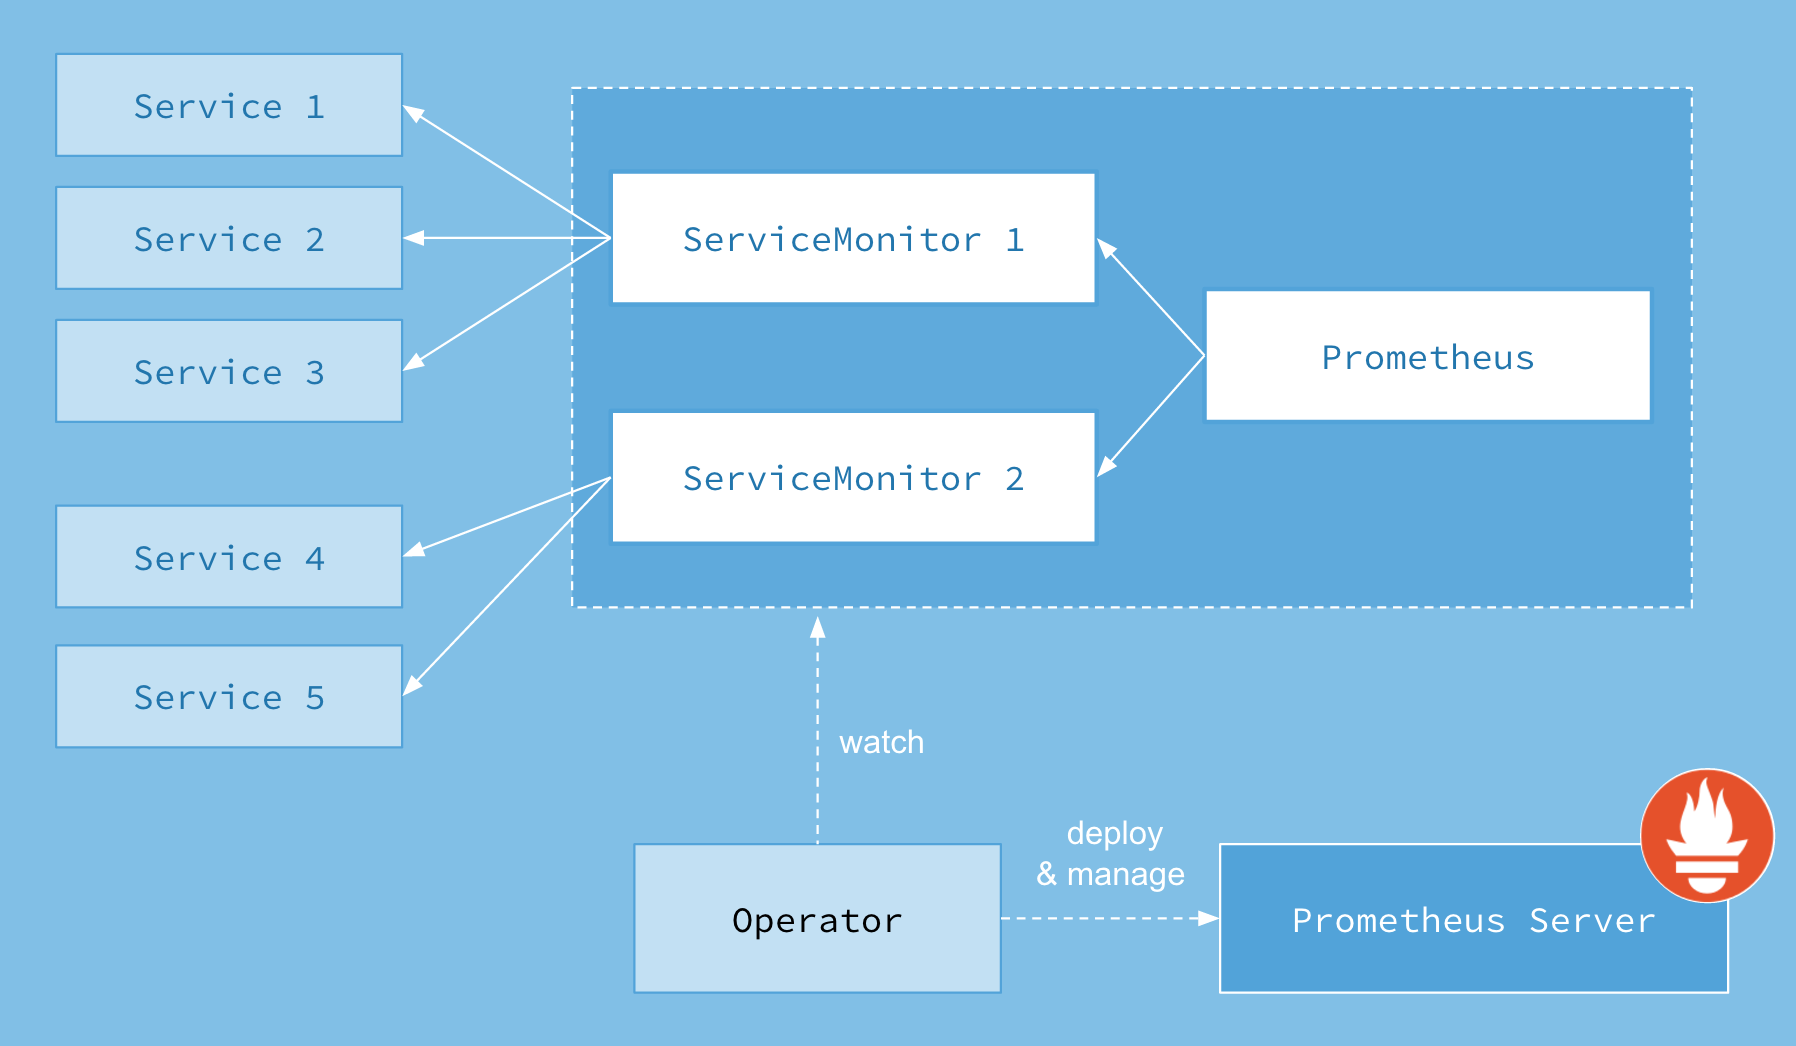
\includegraphics[width=0.5\paperwidth]{Figures/Prom_Operator_Architecture}
%\decoRule
%\caption[Prometheus]{Prometheus Operator Architecture}
%\label{fig:promOpsArch}
%\end{figure}
%*Prometheus Operator Architecture image taken from https://coreos.com/operators/prometheus/docs/latest/user-guides/getting-started.html
%\newpage
\\
\\
\noindent \textbf{Prometheus Operator:} \quad It\footnote{\url{https://coreos.com/operators/prometheus/docs/latest/user-guides/getting-started.html}} creates, configures, and manages Prometheus monitoring instances and, introduces "monitoring" namespace and additional resources Alertmanager and ServiceMonitor to Kubernetes API through \ctexttt{CustomResourceDefinition} (section~\ref{kubeDesign}). The ServiceMonitor uses Kube's Label and Selector to intercept Kubernetes Services (section \ref{kubeService}) and their exposed Prometheus format metrics (i.e. \verb|/metrics|) in evasive way.

\begin{small}
\begin{lcverbatim}
root@athena-kube-master1:~# kubectl get crd
NAME                                    AGE
alertmanagers.monitoring.coreos.com     20d
prometheuses.monitoring.coreos.com      20d
servicemonitors.monitoring.coreos.com   20d
root@athena-kube-master1:~# kubectl get namespaces
NAME          STATUS    AGE
monitoring    Active    20d
root@athena-kube-master1:~# kubectl api-versions|grep monitoring
monitoring.coreos.com/v1
\end{lcverbatim}
\end{small}

\noindent \textbf{Monitoring Setup:} \quad The Metrics Server (Heapster replacement) setup is straight forward. We can create it from the provided manifests as follows.

\begin{small}
\begin{lcverbatim}
root@athena-kube-master1:~# git clone \
		https://github.com/kubernetes-incubator/metrics-server.git
(scrap)
root@athena-kube-master1:~# cd metrics-server
root@athena-kube-master1:~/metrics-server# kubectl create -f deploy/1.8+/
(scrap)
\end{lcverbatim}
\end{small}

Once Metrics Server is up and running, we can observe the cluster wide metrics and monitoring that is scraped from Kubelet Summary API.

\begin{small}
\begin{lcverbatim}
root@athena-kube-master1:~# kubectl api-versions|grep metrics
metrics.k8s.io/v1beta1
root@athena-kube-master1:~# kubectl top node
NAME                  CPU(cores)   CPU%      MEMORY(bytes)   MEMORY%
athena-kube-master1   216m         1%        928Mi           1%
athena-kube-n1        71m          0%        1011Mi          2%
athena-kube-n2        64m          0%        5729Mi          11%
athena-kube-n3        109m         0%        2786Mi          5%
root@athena-kube-master1:~# kubectl top pod
NAME                                CPU(cores)   MEMORY(bytes)
athena-analytics-5ddd588cd6-mv7ff   0m           705Mi
athena-api-server-dc74db874-mk8fp   1m           5462Mi
athena-ui-7f77f68b86-dxf8s          0m           3Mi
athena-worker-79fb4ff6bb-6dns4      1m           1179Mi
athena-worker-79fb4ff6bb-hkjml      1m           1212Mi
---
kubectl get --raw "/apis/metrics.k8s.io/v1beta1/nodes" | python -m json.tool
(scrap)
kubectl get --raw "/apis/metrics.k8s.io/v1beta1/pods" | python -m json.tool
(scrap)
\end{lcverbatim}
\end{small}

The prometheus operator \textbf{Clustering Monitoring} documentation\footnote{\url{https://github.com/coreos/prometheus-operator/blob/master/Documentation/user-guides/cluster-monitoring.md}} provides Kubernetes manifests (i.e. YAMLs) for stetting up the \textbf{Prometheus Operator + kube-prometheus monitoring stack}. However, since the stack comprises of multiple components, it is better to use Helm for the setup.  

\begin{small}
\begin{lcverbatim}
root@athena-kube-master1:~# helm repo add coreos \
	 https://s3-eu-west-1.amazonaws.com/coreos-charts/stable/
"coreos" has been added to your repositories
root@athena-kube-master1:~# helm repo list
NAME  	URL
stable	https://kubernetes-charts.storage.googleapis.com
local 	http://127.0.0.1:8879/charts
coreos	https://s3-eu-west-1.amazonaws.com/coreos-charts/stable/
root@athena-kube-master1:~# helm install coreos/prometheus-operator \
	--name prometheus-operator --namespace monitoring
NAME:   prometheus-operator
(scrap)
\end{lcverbatim}
\end{small}

\noindent \textbf{Helm:} \quad Helm.sh\footnote{\url{https://helm.sh}} is the package manager for Kubernetes. It similar to what APT package management tool to Ubuntu/Debian.

\section{Horizontal Pod Autoscaler}

According to \parencite{kubeDoc}, the Horizontal Pod Autoscaler (HPA) dynamically adjusts the number of Pod replicas in a Deployment based on observed CPU utilisation. It is implemented as a Kubernetes API resource and a controller. To walkthrough, the ATHENA worker deployment manifest as follows.

\begin{small}
\begin{lcverbatim}
apiVersion: apps/v1
kind: Deployment
metadata:
  name: athena-worker
spec:
  selector:
    matchLabels:
      app: athena-worker
  replicas: 2
  template:
    spec:
      containers:
      - name: athena-worker
        image: athena-nexus.eresearch.unimelb.edu.au/athena/athena-worker:latest
(scrap)        
\end{lcverbatim}
\end{small}

\noindent To deploy this:

\begin{small}
\begin{lcverbatim}
kubectl create -f athena-worker.yaml
\end{lcverbatim}
\end{small}

\noindent To scale the deployment:
\begin{small}
\begin{lcverbatim}
kubectl scale deployment athena-worker --replicas=5
\end{lcverbatim}
\end{small}

\noindent Recall (Chapter~\ref{Chapter3}) that this is the similar scaling we did in the plain vanilla Docker-Compose and SWARM stack deployment.

\begin{small}
\begin{lcverbatim}
docker-compose -f docker-compose.yaml -f staging.yaml  --project-name=stg \
   --scale worker=2

docker service scale athena_worker=5   
\end{lcverbatim}
\end{small}

However, with Kubernetes HPA, we can now \textbf{autoscale} the ATHENA worker deployment as follows.
\begin{small}
\begin{lcverbatim}
kubectl autoscale deployment athena-worker --min=1 --max=6 --cpu-percent=80
\end{lcverbatim}
\end{small}

This command\footnote{\url{https://kubernetes.io/docs/reference/kubectl/kubectl/kubectl_autoscale.md}} tells that auto scale a deployment "athena-worker", with the number of Pods between 1 and 6, target CPU utilization at 80\%.

\begin{small}
\begin{lcverbatim}
root@athena-kube-master1:~# kubectl get hpa
NAME            REFERENCE                  TARGETS   MINPODS   MAXPODS   REPLICAS
athena-worker   Deployment/athena-worker   0%/80%    1         6         1    
php-apache      Deployment/php-apache      0%/50%    1         10        1   
\end{lcverbatim}
\end{small}

%\newpage

\noindent Instead of command line, we can also describe the HPA manifest as follow.
\begin{small}
\begin{lcverbatim}
apiVersion: autoscaling/v1
kind: HorizontalPodAutoscaler
metadata:
  name: athena-worker
  namespace: default
spec:
  scaleTargetRef:
    apiVersion: apps/v1
    kind: Deployment
    name: athena-worker
  minReplicas: 1
  maxReplicas: 6
  targetCPUUtilizationPercentage: 80
\end{lcverbatim}
\end{small}

\noindent And, as usual, create the HPA Kubernetes resource object.
\begin{small}
\begin{lcverbatim}
kubectl create -f athena-worker-hpa.yaml
\end{lcverbatim}
\end{small}

The Horizontal Pod Autoscaler feature was introduced in Kubernetes v1.1. The first version of HPA scale the Pod based on observed CPU utilization and memory usage. In Kubernetes 1.6, the Custom Metrics API was introduced that enables HPA access to arbitrary metrics through REST API. In Kubernetes 1.7, the API server aggregation layer allows third party applications to extend the Kubernetes API by registering themselves as API \emph{add-ons}. Note that, the concept about API server aggregation\footnote{\url{https://kubernetes.io/docs/concepts/extend-kubernetes/api-extension/custom-resources/}} is similar to \ctexttt{CustomResourceDefinition} (section~\ref{kubeDesign}), but more flexible. 
%The Custom Metrics API along with the aggregation layer made it possible for monitoring systems like Prometheus to expose application-specific metrics to the HPA controller.

Figure~\ref{fig:kubeMonitAthena} depict the full orchestration of Prometheus metrics monitoring stack with HPA. In Core Metrics pipeline, Metrics Server scrape node and container metrics from Kubelet cAdvisor. In Monitoring pipeline, Prometheus operator collect metrics through its ServiceMonitor and store in Prometheus. And the Grafana dashboard can visual these monitoring metrics. Furthermore, with Prometheus Adapter (an API server aggregation implementation), the Prometheus metrics can be consumed by HPA.

\begin{figure}[H]
\centering
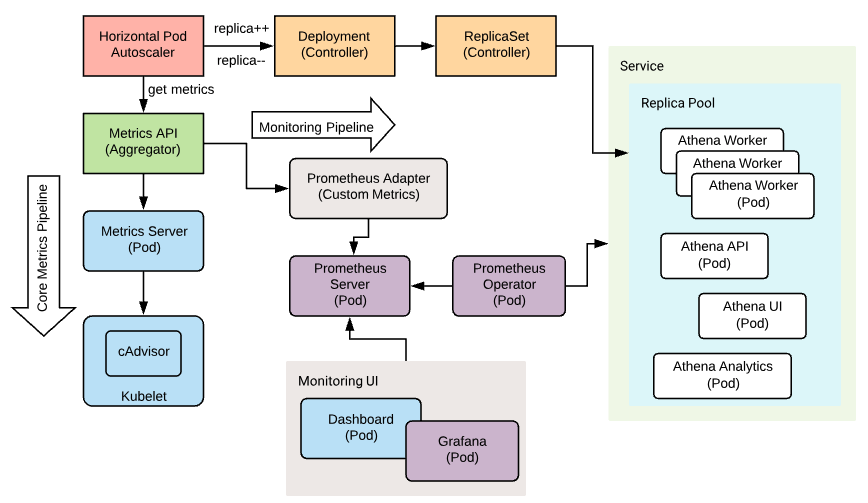
\includegraphics[width=0.7\paperwidth]{Figures/KUBE_monitoring}
\decoRule
\caption[Kubernetes Cluster: HPA and Monitoring for ATHENA]{Kubernetes Cluster: HPA and Monitoring for ATHENA}
\label{fig:kubeMonitAthena}
\end{figure}

\noindent \textbf{HPA Autoscaling Algorithm:} \quad Based on \parencite{kubeDoc}, the HPA implementation of autoscaling algorithm works as follow.

\begin{enumerate}
\item Implemented as a \textbf{Control Loop} - 30 seconds by default, configurable.
\item Periodically queries Pods to collects their CPU utilization
\item Compares the arithmetic mean of the Pods' CPU utilization with the target.
\item Adjusts the replicas of the Scale if needed to match the target, preserving condition: 
	\begin{itemize}
	\item MinReplicas <= Replicas <= MaxReplicas
	\item CPUUtilization (C) = recent CPU usage of a Pod (average across the last 1 minute)  / CPU requested by the Pod (\textit{spec.containers[].resources.requests.cpu}\footnote{\url{https://kubernetes.io/docs/tasks/configure-pod-container/assign-cpu-resource/}})
	\item TargetNumOfPods = ceil(sum(CurrentPodsCPUUtilization) / TargetCPUUtilizationPercentage (T))
	\[ TargetNumOfPods = \left \lceil \left ( \sum_{n=1}^{n} C_{n}  \right )  / T  \right \rceil \]
	\end{itemize}

\item Scale-up can only happen if there was no rescaling within the last 3 minutes. Due to temporarily CPU fluctuation during start/stop.
\item Scale-down will wait for 5 minutes from the last rescaling. Due to temporarily CPU fluctuation during start/stop.
\item Any scaling will only be made if: avg(CurrentPodsConsumption) / TargetCPUUtilizationPercentage drops below 0.9 or increases above 1.1 (10\% tolerance).
\end{enumerate}

\noindent \parencite{kubeDoc} states that algorithm approach has two benefits:
\begin{itemize}
\item Autoscaler works in a conservative way in such that increasing rapidly the number of Pods is important when user load is deteced. However, lowering the number of pods is not that urgent.
\item Autoscaler avoids thrashing, i.e. it prevents rapid execution of conflicting decision if the load is not stable.
\end{itemize}


%% OpenStack node scaling

\newpage

\section{Finding}

Though Kubernetes is complex system to master thoroughly, when in operation, it is found that a very robust and flexible system. There also observable notice in overhead such as service proxies network layer. 

During the experimental runs and it is noticed that the auto-scaler doesn't react immediately to usage spikes. By default the metrics sync happens once every 30 seconds and scaling up/down can only happen if there was no rescaling within the last 3-5 minutes. In this way, the HPA prevents rapid execution of conflicting decisions (oscillation). 

It is also found that auto-scaling based on observed CPU utilisation alone is not sufficient enough for ATHENA worker, due to the dynamic of how the simulation would run: \emph{simulation alone} or \emph{simulation + optimisation}. CPU utilisation scaling works better with optimisation algorithm. However, simulation alone with MONTE CARLO job executed really quick; therefore, miss the scaling observation period delay time and consequently, it missed the HPA replication trigger cycle and there was only 1 worker Pod instance working on jobs -- this could be tune according the target threshold, but it will not be perfect solution. Observing job queue metrics should be implemented.

Figure~\ref{fig:kubeAthena} depict the ATHENA deployment with Kubernetes cluster. Docker Registry is a container image registry hosted using Nexus repository manager.

\begin{figure}[H]
\centering
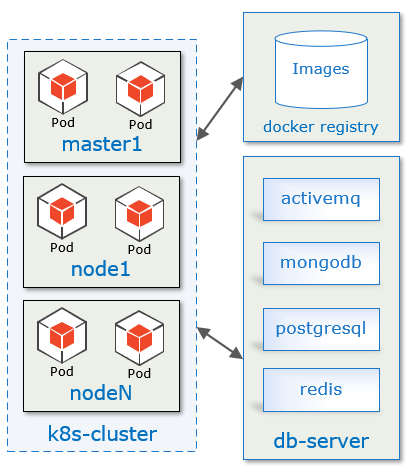
\includegraphics[width=0.5\paperwidth]{Figures/ATHENA_Kube_cluster}
\decoRule
\caption[Kubernetes Cluster ATHENA]{Kubernetes Cluster ATHENA}
\label{fig:kubeAthena}
\end{figure}








 
\chapter{Related Studies and Finding} 

\label{Chapter5} 


The concept of \textit{Auto-Scaling system} is not new. The early research hypothesis dated back to IBM's \textbf{MAPE-K} model discussed in Autonomic Computing \parencite{1160055}. The paper identified the key autonomic elements  -- Monitor, Analyse, Plan, Execute, Knowledge -- the reference model for autonomic control loop for achieving the self-managed (self-optimisation, self-healing) autonomic computing system.

Large-scale cluster management at Google with Borg

Mesos: A Platform for Fine-Grained Resource Sharing in the Data Center

Resource provisioning for data-intensive applications with deadline constraints on hybrid clouds using Aneka

A Comparison of Reinforcement Learning Techniques for Fuzzy Cloud Auto-Scaling





\chapter{Conclusion}

\label{Chapter6}

\section{Conclusion}

In order to produce a reliable auto-scaling system, it is important to understand the target application well, in this case, ATHENA system as discussed in Chapter~\ref{Chapter2}. It is important step to identify which part of system component can be scaled such as ATHENA Worker. It also requires to consolidate the Stateless and Stateful of the system, so that dynamic scaling is possible, as discussed in Chapter~\ref{Chapter3}. It is also crucial to get insight of the foundation platform, Kubernetes as discussed in Chapter~\ref{Chapter4}, to configure properly, get up and running the \emph{Production Ready} cluster. 

Infrastructure scaling on cloud platform required provider specific API and technology. The containerisation deployment with Docker SWARM and Kubernetes technologies can scale across multi-Clouds independently, without the need of Cloud Provider specific API.

Auto-scaling system can not meet SLO and QoS by simply relying on CPU utilisation and memory usage metrics alone. Most web and mobile applications require auto-scaling based on \textit{Requests Per Second} to handle traffic bursts and user load. With new custom metrics API feature introduced in Kubernetes, we can extend the API and expose ATHENA's metrics to Prometheus, then can be consumed by HPA controller and auto-scaled. For enterprise integration system like ATHENA, the auto scaling could be triggered by the ActiveMQ job queue length exceeding some empirical threshold, therefore, Threshold-based reactive approach can be explored.

Effective monitoring and metrics scraping is the heart of the pipeline for auto-scaler to work reliably well. Auto-scaling with Kubernetes is non trivial task to setup for \emph{Production Ready} in Private Cloud, such as NeCTAR Research Cloud.


\section{Future Work}

For the future work, instrumenting ATHENA with Prometheus and exposing the right metrics can fine tune the auto-scaling to better handle bursts, high availability and QoS. We can also explore and design auto-scaling algorithm with different techniques such as Time-series Analysis for Kubernetes as well as implement Docker SWARM based auto-scaler.

We can also explore burstable infrastructure level scaling with OpenStack for NeCTAR and, other Public Cloud Provider. Kubernetes has introduced this in Cloud Manager controller object. For the infrastructure scaling, we can observe the metrics already produced by Kubernetes and Prometheus; and auto-scale nodes based on these metrics.

There are potential comparison and benchmarking studies that can be done within Kubernetes eco-system, such as benchmarking different Pod Networking options, comparison for reliable cluster file systems for Kubernetes, and so on. Highly Available (HA) Kubernetes cluster involves multiple Kube masters; which is interesting space to explore as well.

As for ATHENA, the API backend need to decompose the aggregator component to become a better stateless application, so that it can be scaled well. And to explore ATHENA database stack to deploy it onto Kubernetes cluster using StatefulSet and explore clustered file system store, e.g. Cinder, CephFS, for dynamic volume provision.

%----------------------------------------------------------------------------------------
%	THESIS CONTENT - APPENDICES
%----------------------------------------------------------------------------------------

%\appendix % Cue to tell LaTeX that the following "chapters" are Appendices

% Include the appendices of the thesis as separate files from the Appendices folder
% Uncomment the lines as you write the Appendices

%% Appendix A

\chapter{Appendix} % Main appendix title

\label{AppendixA} % For referencing this appendix elsewhere, use \ref{AppendixA}

%\section{Source Code}
\hfill
\\
\textbf{Source Code Listing}
\\
\hrule
\hfill

\url{https://dstgrp.visualstudio.com/Daenerys/Daenerys Team/_git/deployment}

\url{https://github.com/victorskl/auto-scaling-thesis}

\url{https://github.com/victorskl/kube-node}

\url{https://github.com/victorskl/wharfie}

\url{https://github.com/victorskl/nectar-os-scripts}

\url{https://github.com/victorskl/docker-private-registry}

\url{https://github.com/victorskl/docker-nexus-oss}

\url{https://github.com/victorskl/docker-mongodb}

\url{https://github.com/victorskl/docker-activemq}

\url{https://github.com/victorskl/docker-postgresql}

\url{https://github.com/victorskl/docker-redis}

\url{https://github.com/victorskl/docker-java-beatapp}

\url{https://github.com/victorskl/docker-cplex}

\url{https://github.com/victorskl/spring-boot-tute}
\\
\\
\noindent \textbf{Demo}
\\
\hrule
\hfill

\textit{* Need to be connected on UniMelb VPN}
\hfill

\url{https://115.146.84.84} -- Kubernetes Dashboard

\url{http://115.146.84.84} -- Grafana Dashboard

\url{http://115.146.84.84:9090} -- Prometheus Dashboard

\url{http://115.146.84.84:9093} -- Prometheus Operator Alertmanager

\url{http://115.146.85.147} -- ATHENA UI (Kube Deployment)

\url{http://115.146.85.102/api/swagger} -- ATHENA Data Analytics








%\include{Appendices/AppendixB}
%\include{Appendices/AppendixC}

%----------------------------------------------------------------------------------------
%	BIBLIOGRAPHY
%----------------------------------------------------------------------------------------

\printbibliography[heading=bibintoc]
%\printbibliography

%----------------------------------------------------------------------------------------

\end{document}  
